%%%%%%%%-Metin: Note to Carola: I cannot run bibtex on *blx.aux files on my cpu. Could you please do it for us? (I checked it on another skeleton, the citations are correct) 
%%%%%%%%-Metin: Local packages we use: multirow, gb4e.
%%%%%%%%–Metin: We added the list of abbreviations in the end before the list of references. Hope this is correct.


\documentclass[output=paper]{LSP/langsci} 
\author{Metin Bağrıaçık\affiliation{Ghent University}\and
 Aslı Göksel\affiliation{Boğaziçi University}\lastand 
Angela Ralli\affiliation{University of Patras}
}
\title{Copying compound structures: The case of Pharasiot Greek} 
\abstract{Unlike other Modern Greek dialects in which compounds are one-word structures, in Pharasiot Greek -- an Asia Minor Greek dialect heavily influenced by Turkish -- compounds are formed by two fully inflected words, where the left-hand constituent is marked with compound markers whose shape is conditioned morphologically. Based on  structural similarities between compound structures in Pharasiot Greek and in Turkish, we claim that Pharasiot Greek compounding is selectively copied from Turkish. The compound marker role in Pharasiot Greek is assumed by what are originally genitive suffixes by  identification of the genitive with the Turkish compound marker, which is exapted from a possessive suffix, attaching to right-hand constituent. We correlate certain structural differences between the two languages to the nature and the locus of the compound marker. Among these differences is the occurrence of phrasal constituents in the non-head position in Turkish and lack thereof in Pharasiot Greek. We show that the compound marker in Pharasiot Greek attaches to stems. As such, no phrasal constituent can be hosted in the position to which the compound marker attaches. In Turkish, on the other hand, since the compound marker attaches to the head, the non-head can easily host phrasal constituents. We test this correlation against Khalkha Mongolian, another Altaic language, in which, unlike Turkish, the compound marker attaches to the non-head. We show that similar to Pharasiot Greek, but unlike Turkish, phrasal constituents cannot be hosted in the non-head position in Khalkha, verifying the correlation we proposed between the locus of the compound marker and the availability of phrasal non-heads.}

\ChapterDOI{10.5281/zenodo.885129}



\maketitle

\begin{document} 
\section{Introduction} 
 Despite the recent plethora of research on copying of morphological items (e.g., \citealt{Johanson1992,Gardani2008, Seifart2015b,Seifart2015a,Gardanietal2015} among many others), and the growing interest on structural copying (\citealt{Bowern2008,LepschyTosi2006, Lucas2012,Grimstadetal2014,Lohndal2013,Aboh2015,Thomasonforth}), the question whether compounds are prone to borrowing or not is a topic which still awaits addressing, and copying of compounding has been noted only sporadically, and often as calques (cf. \citealt{Ralli2014}). This seems legitimate as \textit{a priori} it is not clear what can actually be copied as or in a compound since cross-linguistically compounds involve little or no overt functional material.  More importantly, compounding cross-linguistically has an unclear status between \isi{syntax} and morphology (\citealt{Anderson1992,Aronoff1994,DiSciullo2005} among many others, see also \citealt[4--5]{ScaliseVogel2010why} for an overview). As such, it becomes a challenge to make general arguments on what aspects of a compound could be copied. Given the lack of an established cross-linguistic definition of compounds and a consensus on its locus of generation, rather than attempting to make general arguments about (constraints on) `compound copying', a more fruitful approach would be to document cases of `possible compound copying' between languages whose compound structures are relatively well-documented. This is exactly what the current paper aims at. We present a case study of a compound-structure in \ili{Pharasiot Greek} (henceforth PhG), an Asia Minor \ili{Greek} dialect which is on the verge of extinction. We show that compounds in PhG display properties of  two typologically different language systems, i.e., \ili{Turkish} (\ili{Altaic}) and \ili{Greek} (Indo-European).  
 
 As noted by \citet{Ralli2013moderngreek}, typical \ili{Hellenic}\footnote{We refer to all diatopic and diachronic varieties of Modern \ili{Greek} as \ili{Hellenic} in this paper.} compounds involve two lexemes which are concatenated with a compound \isi{marker}, -\textit{o}-, occurring in between the two. These can be attributive, \isi{subordinative} or coordinative compounds. Such compounds are usually inflected as single stems and are \isi{phonological} words bearing single accent.  Although some dialects of Modern \ili{Greek} may not exhibit certain compound types that the others do, across all the modern dialects (\ref{ex:1}),  as well as in older varieties (\ref{ex:2}), the fact that compounds are concatenations of two (or more) lexemes with the compound \isi{marker} -\textit{o}-, i.e., the [X-o-X] template, is constant.\footnote{If there is ever a structural head, it is on the right (cf. \citealt{Ralli2013moderngreek}, see also \citealt{Andreou2014} for exocentric compounds and definition of head in these compounds). This, however, is not exceptionless. In \ili{Ancient Greek} (\ref{ex:2i}) as well as in Modern \ili{Greek} dialect of Bovese (\ref{ex:2ii}) \isi{left-headed} compounds are attested, albeit in a rather limited number in the latter (\citealt{Andreou2014}):
\ea
	\ea\label{ex:2i} \settowidth\jamwidth{(\ili{Ancient Greek})}
		\glll hippop\'{o}tamos\\
			  hipp-o-potamos\\
		      horse-\textsc{cm}-river\\ \jambox{(\ili{Ancient Greek})}
		\glt `hippopotamus' 
	\ex\label{ex:2ii}
		\glll \v{s}\v{s}ul\'{o}furo\\
		      \v{s}\v{s}ul-o-furo\\
		      wood-\textsc{cm}-oven\\ \jambox{(Bovese \ili{Greek}, \citealt[134]{Andreou2014})}
		\glt `wood for oven'
	\z
\z
 }
 
\ea\label{ex:1} 
	\ea\label{ex:1a}\settowidth\jamwidth{(Modern \ili{Greek})}
		\glll	lemonóðendro\\
			    lemon-o-ðendro\\
			    lemon-\textsc{cm}-tree\\ \jambox{(Modern \ili{Greek})}
		\glt	`lemon tree'
	\ex\label{ex:1b} \settowidth\jamwidth{(Cypriot \ili{Greek}, \citealt[132]{Andreou2014})}
		\glll	ampelopérvolon\\
				ampel-o-pervolon\\
				vine-\textsc{cm}-field\\ \jambox{(Cypriot \ili{Greek}, \citealt[132]{Andreou2014})}
		\glt	`vineyard'
	\ex\label{ex:1c} \settowidth\jamwidth{(Pontic \ili{Greek}, \citealt[327]{Papadopoulos1961})}
		\glll	čavdarópsomin\\
				čavdar-o-psomin\\
				rye-\textsc{cm}-bread\\\jambox{(Pontic \ili{Greek}, \citealt[327]{Papadopoulos1961})}
		\glt `rye bread'
	\ex\label{ex:1d} \settowidth\jamwidth{(Aivaliot \ili{Greek}, \citealt{Ralli2016})}
		\glll	ðimunóspurus\\
				ðimun-o-spurus\\
				demon-\textsc{cm}-seed\\ \jambox{(Aivaliot \ili{Greek}, \citealt{Ralli2016})}
		\glt `very smart person'
	\z
\z
	\ea\label{ex:2} \settowidth\jamwidth{(\ili{Ancient Greek}, \citealt[398]{RalliRaftopoulou1999})}
		\glll hoplitódromos\\
				hoplit-o-dromos\\
				hoplite-\textsc{cm}-race\\ \jambox{(\ili{Ancient Greek}, \citealt[398]{RalliRaftopoulou1999})}
		\glt	`Hoplitodromos, race of soldiers'
\z
 
 In PhG, however, this \ili{Hellenic} compounding structure depicted above is absent.\footnote{It should be stated at the outset that in \ili{Cappadocian} \ili{Greek}, a Modern \ili{Greek} dialect closely related to PhG, \ili{Hellenic} compounds are rather restricted. The findings and arguments in this paper may or may not be extended to \ili{Cappadocian} \ili{Greek}. Since we have not investigated compounding in this variety, we will not incorporate such discussion into the current paper.} Instead, PhG compounds are productively formed as concatenations of two lexemes as fully inflected words, whereby the left-hand constituent, the non-head, is marked with a compound \isi{marker}, -\textit{u} or -\textit{s}, depending on the gender of the noun (\ref{ex:3}), whose shape, but not distribution, mirrors that of \isi{genitive} suffixes in the language (\ref{ex:4}):
 
 \begin{multicols}{2}
\ea\label{ex:3}
	\ea\label{ex:3a}
		\glll jorganú xarái\\
				jorgan-\textbf{u} xarai\\
				quilt.\textsc{n}-\textsc{cm} face.\textsc{n.nom.sg}\\
		\glt `quilt cover'
	\ex\label{ex:3b}
		\glll matrákas práða\\
				matraka-\textbf{s} praða\\
				frog.\textsc{f}-\textsc{cm} leg.\textsc{n.nom.pl}\\
		\glt `frog legs'
	\z
\z
\end{multicols}
\ea\label{ex:4}
	\ea\label{4a}
		\glll tu čočuxú ta ɣíða\\
				tu čočux-\textbf{u} ta ɣiða\\
				the.\textsc{n.gen.sg} child.\textsc{n.gen.sg} the.\textsc{n.nom/acc.pl} goat.\textsc{n.nom/acc.pl}\\
		\glt `the child's goats'
	\ex\label{4b}
		\glll s ɣr{\ae}s ta ɣíða\\
				s ɣr{\ae}-\textbf{s} ta ɣiða\\
				the.\textsc{f.gen.sg} beldam.\textsc{f.gen.sg} the.\textsc{n.nom/acc.pl} goat.\textsc{n.nom/acc.pl}\\
		\glt `the beldam's goats'
	\z
\z	
Such concatenations as those in (\ref{ex:3}) can form subordinate and attributive compounds, and unlike all other \ili{Hellenic} varieties, coordinative compounds cannot be formed in this way. The constituents in these compounds retain their own accents, thus causing the compound to behave as a \isi{phonological} phrase in this respect. Besides, such compounds allow limited access to syntactic operations exerted on them, such as external modification of the head or coordination of the constituents. On the other hand, by undergoing \isi{derivation} as single lexical items, or not allowing certain syntactic operations, such as scrambling or outbound anaphora, they behave as lexical items, hence they constitute an example of compounds as borderline cases between phrase-formation and word-formation. 

We interpret the two facts about compounding in PhG, i.e., the lack of \ili{Hellenic} compound structure [X-o-X] and (the emergence of) the productive subordinate or attributive compounds where the non-head is marked with the compound markers -\textit{u} or -\textit{s}, (indicated hereafter as N-\textsc{gen} N, by referring to the similarity of the compound markers to \isi{genitive} suffixes) as one of the many end-products of the heavy and long-lasting influence of \ili{Turkish} on PhG. More specifically, we argue that the N-\textsc{gen} N compound pattern is copied from \ili{Turkish} and incorporated into PhG word formation by evoking native morphological elements. This is verified by a number of interesting common characteristics of \ili{Turkish} N$+$N compounds which are marked at their right periphery by the compound \isi{marker} -\textit{sI}, which itself is \textit{exapted} from a \isi{possessive} \isi{marker}. Since no overt \isi{possessive} markers exist in PhG, the compound \isi{marker} of \ili{Turkish} is identified with the PhG \isi{genitive} \isi{marker}. In other words, the \isi{pattern borrowing} has taken place only selectively.

This selective pattern-borrowing account leads to an interesting question: how much of a pattern can be borrowed between (the) two languages? \ili{Turkish} is known to productively accommodate phrasal strings in the left-hand, i.e., the non-head position of a N$+$N-\textit{sI} compound. If the compound pattern in PhG is indeed borrowed from \ili{Turkish}, then should we also expect the PhG N-\textsc{gen} N compound pattern to be able to accommodate phrasal non-heads? The expectation might be legitimate but it is not confirmed: we will show that nothing of a phrasal sort can be hosted in the non-head position of the PhG N-\textsc{gen} N template, once again verifying that the pattern is only selectively-copied. What renders phrasal non-heads unavailable in this N-\textsc{gen} N requires its own story: We will argue that the morphological affixes employed  as compound markers in the N-\textsc{gen} N template are exapted from native inflectional affixes. Affixes in PhG, as in all other \ili{Hellenic} varieties, attach to bare stems. This is a native rule. Thus, no phrasal element, even when the head of the phrase left-aligns with the \isi{affix}, is a good candidate for this affix-attachment. Hence, the tension between the borrowed pattern and native word-formation rules is resolved by favoring the latter. Thus we see that the pattern is borrowed from \ili{Turkish} but is constrained with native word-formation rules. Then coordination or external modification facts pertinent to the compounds on the one hand and their peculiar atomic behavior on the other require invoking an analysis which can capture such `hybrid' elements between \isi{syntax} and morphology. Without following a strict adherence to any in this paper, we will review certain possible analyses that can capture the peculiarities of these N-\textsc{gen} N compounds as well as their possible locus of generation.

In Section 2 we present a brief overview of \ili{Hellenic} compounding. Section 3 is devoted to the discussion on compounding in PhG and its differences from \ili{Hellenic} compounding. Presenting certain similarities between PhG and \ili{Turkish} in terms of their compound structures, Section 4 argues that the PhG compounding pattern is selectively copied from \ili{Turkish}; however, native functional  material is employed in the pattern. Section 5 delves into phrasal compounds in \ili{Turkish} and lack thereof in PhG and argues that the lack of phrasal non-heads is epiphenomenal on the native compound markers employed in PhG. Section 6 raises some residual questions  about the locus of N-\textsc{gen} N compounding in PhG and provides tentative answers to these questions. Section 7 concludes.

\section{Hellenic compounding}

In a prototypical \ili{Hellenic} compound, two lexemes are juxtaposed with a compound \isi{marker} -\textit{o}- interpolating between the two (\citealt{Ralli2008}). The output, i.e., the compound, is a \isi{phonological} word with a single stress \citep{NesporRalli1994,NesporRalli1996}. The compound \isi{marker} originates from an ancient thematic vowel, but became a compound \isi{marker} already in the Hellenistic period (ca 3rd c. \textsc{bce} -- 3rd c. \textsc{ce}) \citep{AnastasiadiSymeonidi1983,RalliRaftopoulou1999,Ralli2007,Ralli2013moderngreek}. At different periods of the language, the lexemes involved in compounding have been realized as roots or stems, yet at least in Modern \ili{Greek} there is no difference between the two (cf. \citealt[23]{Ralli2005}, \citealt[8]{Ralli2013moderngreek}) and therefore, we will simply use the term `stem' in the rest of the paper. A stem is a lexeme that cannot stand in a syntactic position on its own but can do so only when it is a word, i.e., when it bears (inherent or structural) inflectional material which can be overt or covert. The stems are inflected for gender, case and number, and they are assigned to distinct inflectional classes (\textsc{ic}s) \citep{Ralli2000,Ralli2005}. Such \textsc{ic}s are based on the presence of systematic \isi{stem allomorphy} (for \isi{stem allomorphy} see below) and the form of the entire set of fusional inflectional endings that are combined with the stems. In such a system, gender is a feature inherent to the stems, and nouns of the same gender value may inflect according to different paradigms or conversely, nouns of different gender values may inflect according to the same paradigm. An example of a stem as the representative of \textsc{ic}\oldstylenums{1} is given in Table 1 below.\footnote{Henceforth, stems will be glossed with small capitals and word forms will be written in minuscule.}

\begin{table}
\caption{The declension of the stem `\textit{an}$\theta$\textit{rop}-', `\textsc{human}' (masculine) in \textsc{ic}\oldstylenums{1}.}
\label{table1}
\begin{tabular}{lllllll}
 \lsptoprule
\multirow{2}{*}{Singular} 
& \multicolumn{2}{c}{nominative}      & \multicolumn{2}{c}{accusative}      & \multicolumn{2}{c}{genitive}        \\\cmidrule(lr){2-3}\cmidrule(lr){4-5}\cmidrule(lr){6-7}
                          & stem             & \isi{inflection}       & stem             & \isi{inflection}       & stem             & \isi{inflection}       \\ 
\midrule
% \cline{2-7}
                          & anθrop & -os              & anθrop & -o               & anθrop & -u               \\
                          & \textsc{human}   & -\textsc{nom.sg} & \textsc{human}   & -\textsc{acc.sg} & \textsc{human}   & -\textsc{gen.sg} \\
                          & \multicolumn{2}{c}{`human' (nom.)}   & \multicolumn{2}{c}{`human' (acc.)}   & \multicolumn{2}{c}{`human' (gen.)}   \\ 

\tablevspace 
\midrule
\multirow{2}{*}{Plural}
   & \multicolumn{2}{c}{nominative}      & \multicolumn{2}{c}{accusative}      & \multicolumn{2}{c}{genitive}        \\\cmidrule(lr){2-3}\cmidrule(lr){4-5}\cmidrule(lr){6-7}
                          & stem             & \isi{inflection}       & stem             & \isi{inflection}       & stem             & \isi{inflection}       \\ 
\midrule
% 
% \cline{2-7}
                          & anθrop & -i               & anθrop & -us              & anθrop & -on              \\
                          & \textsc{human}   & -\textsc{nom.pl}  & \textsc{human}   & -\textsc{acc.pl}  & \textsc{human}   & -\textsc{gen.pl}  \\ 
% \cline{2-7}
                          & \multicolumn{2}{c}{`humans' (nom.)}  & \multicolumn{2}{c}{`humans' (acc.)}  & \multicolumn{2}{c}{`humans' (gen.)} \\
                          \lspbottomrule
\end{tabular}
\end{table}

As shown in Table \ref{table1}, the stem \textit{anθrop}- carries the encyclopedic information, `meaning', `gender' and `\textsc{ic}'. In this case it is `masculine' and it belongs to \textsc{ic}\oldstylenums{1}. \textsc{ic}\oldstylenums{1} involves (masculine or feminine) nominals which decline according to the paradigm in Table \ref{table1}. According to \citet{Ralli2000}, there are eight \textsc{ic}s (\textsc{ic}\oldstylenums{1}--\textsc{ic}\oldstylenums{8}) active in Modern \ili{Greek} today. The number of \textsc{ic}s, the way they are structured and which nouns belong to which \textsc{ic}s vary vastly both diachronically and among different dialects; however, for all Modern \ili{Greek} dialects, as far as we can tell, there are \textsc{ic}s and nouns are located in different \textsc{ic}s. 

In a typical \ili{Hellenic} compound, the non-head, i.e., the left hand constituent of a compound is obligatorily a stem (which is formulated as \textit{Bare-Stem Constraint} by \citealt{RalliKarasimos2009}). As for the head position, i.e., the right-hand position of the compound, it can either be occupied by another stem or a word. Hence, the  structures in (\ref{ex:5}) are available in Modern \ili{Greek} as compound structures:
\ea\label{ex:5}
	\ea\label{ex:5a}	\lb{word} \lb{stem} \lb{stem} \textsc{stem} \rb{} -\textsc{cm}- \lb{stem} \textsc{stem} \rb{}\rb{} -\textsc{inflection} \rb{}
	\ex\label{ex:5b}  \lb{word}  \lb{stem} \textsc{stem} \rb{} -\textsc{cm}- \lb{word} \textsc{stem}-\textsc{inflection} \rb{}\rb{}
	
	\hfill \citep[79,~ex.~(9)]{Ralli2013moderngreek}
	\z
\z
 
The structure in (\ref{ex:5a}) is exemplified as (\ref{ex:6a}) and the structure in (\ref{ex:5b}) is exemplified as (\ref{ex:7a}). The compound constituents in their word forms are presented in (\ref{ex:6b}--c) and (\ref{ex:7b}--c) respectively:\footnote{In the following Modern \ili{Greek} examples from this point onwards, we do not provide information about the gender of the stems, which is tangential to the current paper.}

\ea\label{ex:6}
	\ea\label{ex:6a}
		\glll anθropómorfos\\
			anθrop-o-morf-os\\
			\textsc{human}-\textsc{cm}-\textsc{shape}-\textsc{nom.sg}\\
		\glt	`anthropomorphic'
\begin{multicols}{2}
	\ex\label{ex:6b}
		\glll ánθropos\\
				anθrop-os\\
				\textsc{human}-\textsc{nom.sg}\\
		\glt `human'
	\ex\label{ex:6c}
		\glll morfí\\
			morfi-\O \\
			\textsc{shape}-\textsc{nom.sg}\\
		\glt `shape'
	\end{multicols}
	\z
\z

\ea\label{ex:7}
	\ea\label{ex:7a}
		\glll	anθropoθeizmós\\
				anθrop-o-θeizmos\\
				\textsc{human}-\textsc{cm}-\textsc{theism}.\textsc{nom.sg}\\
		\glt	`anthropotheism'
\begin{multicols}{2}
	\ex\label{ex:7b}
		\glll ánθropos\\
				anθrop-os\\
				\textsc{human}-\textsc{nom.sg}\\
		\glt `human'
	\ex\label{ex:7c}
		\glll	θeizmós\\
				θeizm-os\\
				\textsc{theism}-\textsc{nom.sg}\\
		\glt `theism'
\end{multicols}
	\z
\z

Notice that as a reflex of the \textit{Bare-Stem Constraint}, in both (\ref{ex:6a}) and (\ref{ex:7a}), the non-head is a stem (cf. the word forms in (\ref{ex:6b}) and (\ref{ex:7b}) respectively). The compounds in  (\ref{ex:6a}) and  (\ref{ex:7a}) differ, however, as to the shape of the head: in (\ref{ex:6a}), the head of the compound is realized by a stem. This is witnessed by the fact that the inflectional ending of the overall compound in (\ref{ex:6a}), i.e., -\textit{os}, is different than the inflectional ending which the stem in head position would get in isolation (i.e., -\textit{\O}, cf. (\ref{ex:6c})). In other words, the compound stem in (\ref{ex:6a}) is assigned to a different \textsc{ic} than the head noun (i.e., \textit{morf(i)} `shape'). Moreover, the stress of the overall compound is realized on a different syllable than when it falls on its constituents (cf. (\ref{ex:6a}) with (\ref{ex:6b}) and (\ref{ex:6c})). This is formalized as the \textit{Compound Specific Stress Rule} by \citet{NesporRalli1996}, which operates on compounds where both constituents are stems, by assigning the stress to the antepenultimate syllable. Hence, the compound in (\ref{ex:6a}) has the templatic structure shown in (\ref{ex:5a}). In the compound in (\ref{ex:7a}), on the other hand, the head position is realized by a word-form, i.e., a lexeme with its own \isi{inflection}. This is so since the inflectional ending of the compound (\ref{ex:7a}) and of the head word in isolation (\ref{ex:7c}) coincide; in other words, the compound in (\ref{ex:7a}) inherits its \textsc{ic} from its head. Moreover, the stress of the compound and the stress of the head noun in isolation fall on the same syllable (cf. (\ref{ex:7a}) with (\ref{ex:7c})). Hence the compound in (\ref{ex:7a}) is formed on the template in (\ref{ex:5b}).\footnote{The templates in (\ref{ex:5}) are not the only ones operative in Modern \ili{Greek}, nor is the compound type depicted here, i.e., [X-o-X] the sole compound structure. The discussion of all the compound types in Modern \ili{Greek} is well beyond the aims of the current paper. For these cases, the reader is referred to \citet{Ralli2013moderngreek}.}

Another peculiar characteristic of \ili{Hellenic} nouns, which is directly relevant to compound formation, is the phenomenon of \isi{stem allomorphy}. In \ili{Hellenic} varieties, while a certain allomorph of a stem undergoes certain \isi{affixation}, another allomorph of the same lexeme can be employed in other \isi{affixation} processes. To illustrate the case, the lexeme `body' shows this allomorphy between \textit{soma}- and \textit{somat}-. While the former is employed in singular \isi{nominative} and accusative forms, the latter is employed in singular \isi{genitive}, as well as in all the plural forms (see Table \ref{table2}). More relevant to our paper, the latter, i.e., \textit{somat}- is also the one which undergoes \isi{derivation} (\ref{ex:8a}), and can also be employed in certain compounds as a stem (\ref{ex:8b}, \ref{ex:8c}):

\begin{table}
\caption{\textit{soma-} {\textasciitilde} \textit{somat-} (neuter) `\textsc{body}' stem allomorphy in \textsc{ic}\oldstylenums{8}}
\label{table2}
\begin{tabularx}{.75\textwidth}{Xllll}
 \lsptoprule
           & \multicolumn{2}{c}{singular} & \multicolumn{2}{c}{plural} \\
\midrule
{nominative} & soma           & -\O         & somat         & -a         \\
{accusative} & soma           & -\O         & somat         & -a         \\
{genitive}   & somat          & -os         & somat         & -on        \\
\lspbottomrule      
\end{tabularx}
\end{table}

\ea\label{ex:8}
	\ea\label{ex:8a}
		\glll 	somatíðio\\
				somat-iði-o\\
				\textsc{body}-\textsc{der}-\textsc{nom.sg}\\
		\glt	`particle; corpuscle'
\begin{multicols}{2}
	\ex\label{ex:8b}
		\glll	somatofílakas\\
				somat-o-filakas\\
				\textsc{body-cm-guard.nom.sg}\\
		\glt	`bodyguard'
	\ex\label{ex:8c}
		\glll	kiknosómatos\\
				kikn-o-somat-os\\
				\textsc{swan-cm-body-nom.sg}\\
		\glt	`swan-bodied'
\end{multicols}
	\z
\z

Note that  in a few cases, the other stem, i.e., \textit{soma}-, can also be employed in a compound (see 8d below). In this case, at first glance it is not clear whether the lexeme employed in the head position is the stem or the word form of the lexeme since their overt forms coincide when the word is in \isi{nominative} case (cf. Table \ref{table2}). The difference in the position of stress between the compound and the head noun in isolation, however, suggests that the form employed is a stem (cf. the stress on the compound in (8d) and the stress on the head constituent in isolation 8e):\footnote{If the compound head is a word, it always retains its own stress. See \citet{Ralli1988}, where the location of word stress in Modern \ili{Greek} is morpho-phonologically accounted for. }
\begin{multicols}{2}
\begin{exe}
\exi{(8)}
\begin{xlist}
	\exi{d.}\label{ex:8d}
		\glll	xromósoma\\
				xrom-o-soma-{\O} \\
				\textsc{color-cm-body-nom.sg}\\
		\glt	`chromosome'
		
	\exi{e.}\label{ex:8e}
		\glll	sóma\\
				soma-{\O} \\
				\textsc{body-nom.sg}\\
		\glt	`body'	
	
\end{xlist}
\end{exe} 
\end{multicols}

The structures presented as templates in (\ref{ex:5}) are highly productive in standard Modern \ili{Greek} and in most Modern \ili{Greek} varieties, and the permutations allowed are the following: N$+$N, A$+$A, V$+$V, A$+$N, N$+$V, Adv$+$V which are exemplified in (\ref{ex:9}--\ref{ex:14}) respectively:
\ea\label{ex:9} N$+$N (stem $+$ word)
	\ea\label{ex:9a}
		\glll	anθropoθeizmós\\
				anθrop-o-θeizmos\\
				\textsc{human}-\textsc{cm}-\textsc{theism}.\textsc{nom.sg}\\
		\glt	`anthropotheism'
\begin{multicols}{2}
	\ex\label{ex:9b}
		\glll ánθropos\\
				anθrop-os\\
				\textsc{human}-\textsc{nom.sg}\\
		\glt `human'
	\ex\label{ex:9c}
		\glll	θeizmós\\
				θeizm-os\\
				\textsc{theism}-\textsc{nom.sg}\\
		\glt `theism'
\end{multicols}
	\z
\z
\ea\label{ex:10} A$+$A (stem $+$ stem)\begin{multicols}{2}
	\ea\label{ex:10a}
		\glll 	asprómavros\\
				aspr-o-mavr-os\\
				\textsc{white-cm-black-nom.sg}\\
		\glt	`black and white'

	\ex\label{ex:10b}
			\glll	áspros\\
					aspr-os\\
					\textsc{white-nom.sg}\\
			\glt	`white'
	\ex\label{ex:10c}
			\glll mávros\\
					mavr-os\\
					\textsc{black-nom.sg}\\
			\glt	`black'

	\z\end{multicols}
\z
\ea\label{ex:11} V$+$V (stem $+$ word)
	\ea\label{ex:11a}
		\glll	anavosvíno\\
				anav-o-svin-o\\
				\textsc{turn.on-cm-turn.off-1sg}\\
		\glt	`I turn on and off'
\begin{multicols}{2}
	\ex\label{ex:11b}
		\glll	anávo\\
				anav-o\\
				\textsc{turn.on-1sg}\\
		\glt	`I turn on'
	\ex\label{ex:11c}
		\glll svíno\\
				svin-o\\
				\textsc{turn.on-1sg}\\
		\glt	`I turn off'
\end{multicols}
	\z
\z
\ea\label{ex:12} A$+$N (stem$+$word)
	\ea\label{ex:12a}
		\glll kalóɣeros\\
				kal-o-ɣer-os\\
				\textsc{good-cm-old.man-nom.sg}\\
		\glt	`monk'
\begin{multicols}{2}
	\ex\label{ex:12b}
		\glll	kalós\\
				kal-os\\
				\textsc{good-nom.sg}\\
		\glt	`good'
	\ex\label{ex:12c}
		\glll ɣéros\\
				ɣer-os\\
				\textsc{old.man-nom.sg}\\
		\glt	`old man'
\end{multicols}
	\z
\z
\ea\label{ex:13} N$+$V (stem $+$ word)
	\ea\label{ex:13a}
		\glll laɣokimáme\\
				laɣ-o-kim-ame\\
				\textsc{hare-cm-sleep-1sg}\\
		\glt	`I doze'
\begin{multicols}{2}
	\ex\label{ex:13b}
		\glll	laɣós\\
				laɣ-os\\
				\textsc{hare-nom.sg}\\
		\glt	`hare'
	\ex\label{ex:13c}
		\glll	kimáme\\
				kim-ame\\
				\textsc{sleep-1sg}\\
		\glt	`I sleep'
\end{multicols}
	\z
\z
\ea\label{ex:14} Adv$+$V (stem $+$ word)
	\ea\label{ex:14a}
		\glll krifokitázo\\
				krif-o-kitaz-o\\
				\textsc{secret-cm-look-1sg}\\
		\glt	`I peek'
\begin{multicols}{2}
	\ex\label{ex:14b}
		\glll	krifá\\
				krif-a\\
				\textsc{secret-adv}\\
		\glt	`secretly'
	\ex\label{ex:14c}
		\glll	kitázo\\
				kitaz-o\\
				\textsc{look-1sg}\\
		\glt	`I look'
\end{multicols}
	\z
\z
The information we provided above concerning \ili{Hellenic} compounding might be the tip of an iceberg to the interested reader. However, this information is sufficient for the purposes of the current paper. For a more detailed account of compounding in (Modern) \ili{Greek}, we refer the reader to \citet{Ralli2013moderngreek}.

\section{Compounding in Pharasiot Greek}
The dialect of Pharasa, along with the dialects spoken in Cappadocia, Pontus and Silli, is an Asia Minor \ili{Greek} dialect which was spoken in at least seven villages in the southeast Kayseri province and north of Adana province of modern-day Turkey, in the area known also as Pharasa \citep{Dawkins1916} until 1923. In the years following 1923, the PhG speaking population was relocated to a few villages in Northern Greece according to the population exchange that was enacted as a supplementary protocol to the Treaty of Lausanne signed in 1923. The exact number of speakers before the population exchange is difficult to state as the accounts pertinent to the population of Pharasa also include the \ili{Turkish}-speaking Orthodox population of the region. Based on earlier accounts \citep{Xenofanis,Sarantidis1899,Kyrillos,Dawkins1916}, \citet{Bagriacik} estimates that the number of PhG speakers before the population exchange was around 2000. Today, the dialect is spoken by about 25  second generation refugees in a few villages of Northern Greece. The dialect has long been assigned an unclear status, such as being a sub-dialect of Pontic (cf. \citealt{Dawkins1916}, \citealt[27]{Dawkins1937}), which nevertheless has curious connections with the dialect of Cyprus \citep[22]{Dawkins1940}. It is also often treated as a variant of \ili{Cappadocian} \citep{Anastasios1976}, justified mostly by its geographical proximity to Cappadocia. The growing interest in micro-comparative work on \ili{Greek} dialects and work especially on PhG, however, reveals that PhG must have diverged at a much earlier time-period than \ili{Cappadocian} and Pontic (\citealt{Karatsareas2011}, \citealt{Bagriacik}). Similar to other Asia Minor \ili{Greek} dialects, PhG has been isolated from the rest of the \ili{Greek} speaking world possibly in the early Medieval \ili{Greek} period, and it had been heavily influenced by (Old) Anatolian \ili{Turkish} at all levels of grammar. The dialect was also influenced by the neighboring \ili{Armenian} dialects, though mostly at the lexical level. Beside retentions or innovations common to all Asia Minor \ili{Greek} dialects, the dialect also exhibits remarkable differences from the rest of the Asia Minor \ili{Greek} dialects at all levels of its grammar. Since the speakers of PhG have been living in Greece for the last 90 years, and are thus bilinguals in Standard \ili{Greek} and PhG, the influence of Modern \ili{Greek} is also observed in certain domains (see \citealt{Bagriacik}).

Of the numerous peculiar properties of PhG, one is the lack of prototypical \ili{Hellenic} compounding depicted in section 2. The collections in the dialect both prior to the population exchange (e.g., \citealt{Lagarde1886,Levidis1892,Gregoire1909,Dawkins1916}) or texts written in and on the dialect after the population exchange (e.g., \citealt{Theodoridis1960,Theodoridis1964,Theodoridis1966}) contain no tokens of \ili{Hellenic}-style compounding [X-o-X]. A recent dictionary of the dialect \citep{Papastefanou2012} contains only a few instances of [X-o-X] compounds, which, however, seem to be borrowed from Modern \ili{Greek} since they belong to medical or scientific jargons:
\ea\label{ex:15}
	\glll emoréja\\
			em-o-reja\\
			\textsc{blood-cm-burst.f.nom.sg}\\
	\glt `hemorrhaging'\hfill (cf. Modern \ili{Greek}, \textit{emoréja})
\z \largerpage[]
This, however, does not mean that compounding is missing altogether in the dialect. There is a  productive N+N compound structure in which both the head, i.e., the right hand constituent, and the non-head, i.e., the left-hand constituent, are word forms.\footnote{Such examples abound in the dictionary by \citet{Papastefanou2012}. However, the indication of stress in these compounds is arbitrary; sometimes it is shown only once, sometimes both are indicated and sometimes they are omitted altogether. We assume that this is either because PhG does not have a uniform orthographic convention, or the \isi{stress pattern} was unknown to the authors.}\textsuperscript{,}\footnote{There are also certain attributive A$+$N combinations (\ref{ex:9i}), or N$+$N combinations (\ref{ex:9ii}) as coordinate structures that are possible candidates for compounding. These structures, however, do not involve a compound \isi{marker} and both constituents bear their own \isi{inflection} and stress (see \citealt{Bagriacik} and \citealt{Bagriaciketalforthcoming} for further details.):

\ea\label{ex:9i}
	\gll 	traxariéris nomáts\\
			hairy.\textsc{m.nom.sg} man.\textsc{m.nom.sg}\\
	\glt	`ogre'
\z
\ea\label{ex:9ii}
	\gll	ma tatá\\
			mother.\textsc{f.nom/acc.sg} father.\textsc{m.nom/acc.sg}\\
	\glt	`mother-father'
\z
We will not discuss the structures in (\ref{ex:9i}--\ref{ex:9ii}) in the current paper.
}

However, the \isi{inflection} of the non-head constituent varies according to the gender of the base that it attaches to. Similar to  Modern \ili{Greek},  PhG nouns, simplex or complex (i.e., compounds or derived words), are assigned to different \textsc{ic}s. While masculine and neutral nouns of various \textsc{ic}s are affixed with -\textit{ú} (\ref{ex:16a}), feminine nouns of various \textsc{ic}s are affixed with -\textit{s} (\ref{ex:17a}). These suffixes are also employed for expressing the \isi{genitive}  in masculine/neuter and feminine nouns respectively (cf. (\ref{ex:18a}) and (\ref{ex:18b})):
\ea\label{ex:16}
	\ea\label{ex:16a}
		\glll	zejtinú álima \\
				zejtin-u alima-\O \\
				\textsc{olive.n-cm} \textsc{oil.n-nom.sg}\\
		\glt `olive oil'
\begin{multicols}{2}
	\ex\label{ex:16b}
		\glll	zejtín\\
				zejtin-\O \\
				\textsc{olive.n-nom.sg}\\
		\glt	`olive'
	\ex\label{ex:16c}
		\glll	álima\\
				alima-\O \\
				\textsc{oil.n-nom.sg}\\
		\glt	`oil'
\end{multicols}    
	\z
\z   
\ea\label{ex:17}
	\ea\label{ex:17a}
		\glll	matrákas práði\\
				matraka-s práði-\O \\
				\textsc{frog.f-cm} \textsc{leg.n-nom.sg}\\
		\glt	`frog leg'
\begin{multicols}{2}
	\ex\label{ex:17b}
		 \glll	matráka\\
		 		matraka-\O \\
		 		\textsc{frog.f-nom.sg}\\
		 \glt	`frog'
	\ex\label{ex:17c}
		\glll	práði\\
				praði-\O\\
				\textsc{leg.n-nom.sg}\\
		\glt	`leg'
\end{multicols}
	\z
\z
\ea\label{ex:18}
	\ea\label{ex:18a}
		\glll tu  zejtinú  o fajdás\\
				tu zejtin-u o fajda-s\\
				the.\textsc{n.gen.sg} \textsc{olive.n-gen.sg} the\textsc{.nom.sg} \textsc{benefit.m-nom.sg}\\
		\glt `the benefit of the olive'
	\ex\label{ex:18b}
		\glll s matrákas ta ftálm{\ae}\\
				s matraka-s ta ftalm-{\ae}\\
				the.\textsc{f.gen.sg} \textsc{frog.f-gen.sg} the.\textsc{n.nom/acc.pl} \textsc{eye}.\textsc{n-nom/acc.pl}\\
		\glt `the frog's eyes'
	\z
\z
Therefore, at first glance it might be stated that -\textit{u} or -\textsc{s} are \isi{genitive} markers in (\ref{ex:16})--(\ref{ex:17}) similar to the case in (\ref{ex:18}), and the structures in  (\ref{ex:16})--(\ref{ex:17}) are thus not compounds but indefinite/non-specific genitives. Below, we will provide detailed evidence for the fact that the structures in  (\ref{ex:16})--(\ref{ex:17}) are indeed compounds, behaving differently than the phrases in (\ref{ex:18}); however, for the time being, let us show that this view is in error by stating that the structure exemplified in  (\ref{ex:16})--(\ref{ex:17}) can also generate compounds where the constituents are not in a possession relation (\ref{ex:19a}).  	Moreover, attributive compounds (in the sense of \citealt{ScaliseBisetto2009}) can also be formed based on the same template (\ref{ex:19b}):
\ea\label{ex:19}
	\ea\label{ex:19a}
		\glll pejgirú mamútsi\\
				pejgir-u mamutsi-\O \\
				\textsc{horse.n-cm} \textsc{fly.n-nom.sg}\\
		\glt `horse fly'
	\ex\label{ex:19b}
		\glll θalú tupéki\\
				θal-u tupeki-\O \\
				\textsc{stone.n-cm} \textsc{mortar.n-nom.sg}\\
		\glt `stone mortar'
	\z
\z
Note that the \isi{genitive} phrasal counterpart of (\ref{ex:19a}) in (\ref{ex:20}) does not show the semantic integrity that (\ref{ex:19a}) does; rather it refers to a discourse-salient entity:
\ea\label{ex:20}
	\glll tu pejgirú to mamútsi\\
			tu	pejgir-u to mamutsi-\O \\
			the.\textsc{n.gen.sg}	\textsc{horse.n-cm} the.\textsc{n.nom/acc.sg} \textsc{fly.n-nom.sg}\\
		\glt `the fly of the horse'
\z
Moreover, PhG \isi{genitive} phrases in (\ref{ex:18}) and (\ref{ex:20}) clearly differ from the N-\textsc{gen} N compound structures (\ref{ex:16})--(\ref{ex:17}) by the fact that in a \isi{genitive} phrase the \isi{genitive} article is obligatory: 
\ea\label{ex:21}
	\glll *(tu) zejtinú  o/an fajdás\\
			*(tu) zejtin-u o/an fajda-s\\
				the.\textsc{n.gen.sg} \textsc{olive.n-gen.sg} the\textsc{.nom.sg}/a \textsc{benefit.m-nom.sg}\\
		\glt `the/a benefit of the olive'
\z
By not involving this \isi{genitive} article, the structures in (\ref{ex:16})–(\ref{ex:17}) and (\ref{ex:19}) diverge from \isi{genitive} phrases.

More important evidence for the fact that structures built on the N-\textsc{gen} N template are not \isi{genitive} phrases comes from a group of masculine nouns which receive the –\textit{u} \isi{suffix} only when they are in the non-head position of a compound (\ref{ex:22}). When they are in a \isi{genitive} phrase, the \isi{suffix} marking the \isi{genitive} is zero (\O) (\ref{ex:23}):
\ea\label{ex:22}
	\glll ɣɯjmaðú koftéða\\
			ɣɯjmað-u kofteð-a\\
			\textsc{ground.meat.m-cm} \textsc{meatball.m-nom.pl}\\
	\glt `(a type of) meatballs'
\z
\ea\label{ex:23}
	\glll tu ɣɯjmá i  muruðía\\
			tu ɣɯjma-{\O} i muruðia-\O\\
			the.\textsc{m.gen.sg} \textsc{ground.meat.m-gen.sg} the.\textsc{f.nom.sg} \textsc{smell.f-nom.sg}\\
	\glt `the smell of the ground meat'
\z
The difference in the stem choice in (\ref{ex:22}) and (\ref{ex:23}) is an instance of \isi{stem allomorphy} in PhG as \textit{ɣɯjma-} {\textasciitilde} \textit{ɣɯjmað-} , identical to \isi{stem allomorphy} in Modern \ili{Greek} (cf. Section 2). It is the stem \textit{ɣɯjmað-} which is employed in compounding. The same stem is also employed in plural \isi{inflection}, while \textit{ɣɯjma-} receives singular inflectional suffixes. This latter point is exemplified by another lexeme of the same \textsc{ic}, \textit{zopa}-  {\textasciitilde} \textit{zopað}- ‘\textsc{stove}’ in Table \ref{table3} below:
\begin{table}[h!]
\caption{\textit{zopa-} {\textasciitilde} \textit{zopa$\delta$-} (neuter) `\textsc{stove}' stem allomorphy in PhG (corresponding to \textsc{ic2} of Modern Greek)}
\label{table3}
\begin{tabularx}{.75\textwidth}{XlXlX}
 \lsptoprule
           & \multicolumn{2}{l}{singular} & \multicolumn{2}{l}{plural} \\
\midrule
{nominative} & zopa           & -s         & zopað         & -i         \\
{accusative} & zopa           & -\O        & zopað         & -i         \\
{genitive}   &  zopa          & -\O        & zopað         & -i/iun        \\
\lspbottomrule      
\end{tabularx}
\end{table}

If genuine \isi{genitive} suffixes were employed when (masculine) nouns of \textsc{ic}\oldstylenums{2} are in the non-head position of a compound, then in (\ref{ex:22}) we would expect the zero \isi{genitive} \isi{marker} (\O), and not -\textit{u}, contrary to fact.\footnote{There is another possible account for the –\textit{u} attaching to \textsc{ic2} stems in PhG, which ultimately cannot be maintained:

Such \textsc{ic2} stems can occur in the non-head position of a compound, not only in PhG but in Modern \ili{Greek} or in other dialects as well. Consider (\ref{ex:10i}) and (\ref{ex:10ii}) which are from Modern \ili{Greek} and Lesbian/Aivaliot respectively:
\begin{multicols}{2}
\ea\label{ex:10i}
	\glll 	kimaðomixaní\\
			kimað-o-mixani\\
			\textsc{ground.meat-cm}-machine\\
	\glt	`meat grinder'
\z
\ea\label{ex:10ii}
	\glll	kimaðumixaní\\
			kimað-u-mixani\\
			\textsc{ground.meat-cm}-machine\\
	\glt	`meat grinder'
\z
\end{multicols}
The only difference between (\ref{ex:10i}) and (\ref{ex:10ii}) is the fact that in (\ref{ex:10ii}), which is from Lesbian/Aivaliot, the compound \isi{marker} is realized not as -\textit{o}-, but as -\textit{u}-. This, however, is only due to a \isi{phonological} process in Northern \ili{Greek} dialects, namely the raising of unstressed [o] to [u], cf. \citet{Chatzidakis1905}. In fact, such raising of unstressed [o] to [u] occurs in some villages of Pharasa, albeit not systematically, contrary to the case in Northern \ili{Greek} dialects where the raising takes place across the board. Still, the -\textit{u} attaching to \textsc{ic2} stems in PhG (or to stems of any IC for that matter) might be argued not to be a genuine \isi{suffix} exapted from the \isi{genitive}, but to be underlyingly the compound \isi{marker} [o], raised to [u]. This, however, cannot be maintained, since -\textit{u} is always stressed (cf. (\ref{ex:22})) and for [o] $>$ [u]  raising to take place -\textit{u}, which, according to the scenario, is the hypothetical compound \isi{marker} -\textit{o}-, should have been unstressed.
} Therefore, we argue that the compound structure N-\textsc{gen} N is not a \isi{genitive} phrase (see also  below for more structural differences between the two). Concomitantly, the -\textit{u} and -\textit{s} suffixes are not genuine \isi{genitive} suffixes in the template N-\textsc{gen} N. This means that they are in fact compound markers marking the process of compounding in PhG, which are exapted from the \isi{genitive} suffixes, where \textit{exaptation} should be defined as an unpredictable and leap-like shift of the function of a specific morpheme (\citealt[8]{Nordevandevelde2016}). This is another difference between \ili{Hellenic} compounding and PhG compounding: while in the former the compound \isi{marker} is exapted from an ancient thematic vowel (see Section 2), PhG compounds are marked by compound markers exapted from the \isi{genitive} and are sensitive to the gender of the base they attach to. 

Another salient difference between \ili{Hellenic} compounding and PhG compounding lies in the stress. As was discussed in Section 2, \ili{Hellenic} compounds are \isi{phonological} words. The stress falls on the stressed syllable of the head if the lexeme occupying the head position is a word. Otherwise, the \textit{Compound Specific Stress Rule} positions the stress on the antepenultimate syllable. In either case, though, the whole juxtaposition has single stress. In PhG compounds, on the other hand, both constituents retain their own stress, hence the whole concatenation acts as a \isi{phonological} phrase. While the primary accent falls on the stressable syllable of the non-head, the head carries a secondary stress. Hence the \isi{stress pattern} of PhG compounds resembles that of respective \isi{genitive} phrases (if there is a corresponding \isi{genitive} phrase). The figures in (\ref{ex:24b}) and (\ref{ex:25b}) show the resemblance of the stress patterns of compounds and \isi{genitive} phrases respectively (where the leftmost constituent receives main stress):\footnote{Hereafter, in order to avoid redundant morphemic glossing, we will not provide gender, case or number information in the examples when they do not directly affect the discussion.} 
\ea\label{ex:24}
	\ea\label{ex:24a}
		\glll ((matrákas)$_{\omega}$ (práða)$_{\omega}$)$_{\phi}$ \\
				matraka-s praða\\
				\textsc{frog-cm} legs\\
		\glt `frog legs'
	\ex\label{ex:24b}
 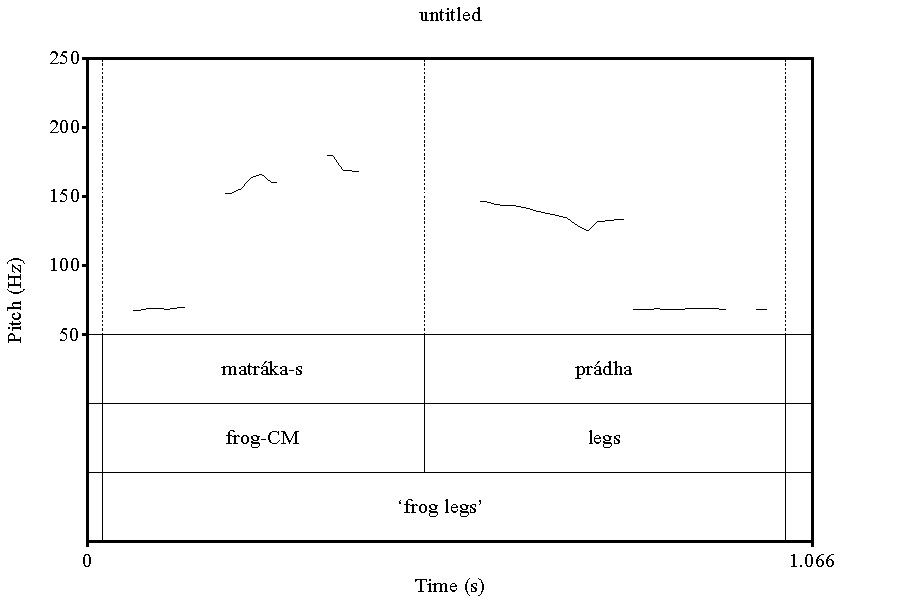
\includegraphics[scale=0.50,valign=t]{figures/matrakas.pdf}
	\z
\z
\ea\label{ex:25}
	\ea\label{ex:25a}
		\glll  ((s matrákas)$_{\omega}$ (ta práða)$_{\omega}$)$_{\phi}$ \\
				s matraka-s ta praða\\
				the.\textsc{gen} frog-\textsc{gen} the legs\\
		\glt `the frog's legs'
	\ex\label{ex:25b}
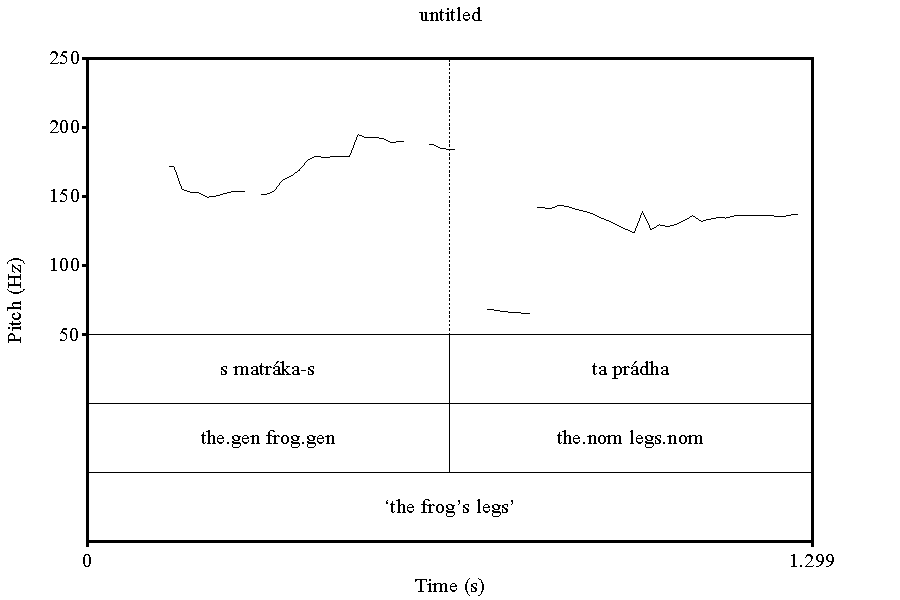
\includegraphics[scale=0.50,valign=t]{figures/matrakas2.pdf}
	\z
\z

The affinity of compounds in PhG to \isi{genitive} phrases is not only witnessed by the origin and the gender-sensitivity of the compound markers, and the \isi{phonological} phrasehood of the compound. N-\textsc{gen} N compounds also behave similar to \isi{genitive} phrases in certain syntactic constructions. Such behavior again clearly sets them apart from \ili{Hellenic} compounds which show no affinity with phrases.

\ili{Hellenic} compounds are known not to allow any syntactic operation on their structure \citep{Ralli2007,Ralli2013moderngreek}; for example, the constituents in a \ili{Hellenic} compound cannot be coordinated. Compare the ungrammatical \isi{coordinate structure} in (\ref{ex:26}) to \isi{grammatical} compounds in (\ref{ex:27}):  

\ea[*]{\label{ex:26}
	\glll vamvakkekapnoxórafo\\
          vamvak-ke-kapn-o-xoraf-o\\
          \textsc{cotton}-and-\textsc{tobacco-cm-field-nom.sg}\\ \jambox{(Modern \ili{Greek})}
      \glt  int.: `cotton and tobacco field'
      }
\z
\begin{multicols}{2}
\ea\label{ex:27}
	\ea\label{ex:27a}
		\glll vamvakoxórafo\\
				vamvak-o-xoraf-o\\
				\textsc{cotton-cm-field-nom.sg}\\
		\glt	`cotton field'
	\ex\label{ex:27b}
		\glll	kapnoxórafo\\
				kapn-o-xoraf-o\\
				\textsc{tobacco-cm-field-nom.sg}\\
		\glt	`tobacco field'
	\z
\z
\end{multicols}

PhG compounds, on the other hand, allow for the coordination of compound non-heads. In (\ref{ex:28}), the non-head is coordinated, and the whole structure has a unique denotation; a field where both barley and alfalfa are planted (biennially due to the toxicity of the latter):
\ea\label{ex:28}
	\glll kočú če rovú tópus\\
			koč-u če rov-u topus\\
			\textsc{barley-cm} and \textsc{alfalfa-cm} field\\
	\glt `a field where barley and alfalfa are planted'
\z

However, the possibility for the non-head to host a \isi{coordinate structure} correlates with the degree of semantic compositionality of the compound. In (\ref{ex:29a}), for example, the coordination of the non-head results in an ungrammatical structure:
\ea\label{ex:29}
	\ea[*]{\label{ex:29a}
		\glll 	širiðú če nékas čarúxa\\
				širið-u če neka-s čaruxa\\
				\textsc{pig-cm} and \textsc{woman-cm} shoes\\
		\glt int.: `shoes made from pigskin and women's shoes'
}
\begin{multicols}{2}
	\ex\label{ex:29b}
		\glll	širiðú čarúxa\\
				širið-u čaruxa\\
				\textsc{pig-cm} shoes\\
		\glt `shoes made from pigskin'
	\ex\label{ex:29c}
		\glll nékas čarúxa\\
				neka-s čaruxa\\
				\textsc{woman-cm} shoes\\
		\glt `women's shoes'
\end{multicols}
	\z
\z
The ungrammaticality is arguably due to the fact that the same thematic role could not be  mapped onto both non-heads in (\ref{ex:29a}). The same results obtain in coordination of the head. In (\ref{ex:30a}), where the same thematic relationship occurs between the non-head and the heads, coordination of the head is acceptable. In (\ref{ex:31a}), however, coordination is ungrammatical:
\ea\label{ex:30}
	\ea\label{ex:30a}
		\glll	ɣuvalú čeratú če petsí\\
				ɣuval-u čeratu če petsi\\
				\textsc{water.buffalo-cm} horn and skin\\
			\glt `water buffalo horn and skin'
\begin{multicols}{2}
	\ex\label{ex:30b}
		\glll	ɣuvalú čeratú \\
				ɣuval-u čeratu\\
				\textsc{water.buffalo-cm} horn\\
		\glt `water buffalo horn'
	\ex\label{ex:30c}
		\glll	ɣuvalú petsí\\
				ɣuval-u petsi\\
				\textsc{water.buffalo-cm} skin\\
		\glt `water buffalo skin'
\end{multicols}
	\z
\z
\ea\label{ex:31}
	\ea[*]{\label{ex:31a}
		\glll	ɣaiðurú gafás če melísi\\
				ɣaiður-u gafas če melisi\\
				\textsc{donkey-cm} head and bee\\
		\glt int.: `yackety-yak and wasp'}
\begin{multicols}{2}
	\ex\label{ex:31b}
		\glll	ɣaiðurú gafás\\
				ɣaiður-u gafas\\
				\textsc{donkey-cm} head\\
		\glt `yackety-yak'
	\ex\label{ex:31c}
		\glll ɣaiðurú melísi\\
				ɣaiður-u melisi\\
				\textsc{donkey-cm} bee\\
		\glt `wasp'
\end{multicols}
	\z
\z
As far as we can tell, \textit{ke} `and' in \ili{Hellenic} varieties is a phrasal coordinator (see \citealt{Ingria2005} for Modern \ili{Greek}). \textit{\v{C}e} `and' in PhG, which is ultimately the \ili{Hellenic} \textit{ke}, is, similarly, a phrasal coordinator. In (\ref{ex:32}) below, two  \isi{genitive} phrases are coordinated with \textit{\v{c}e}:
\ea\label{ex:32}
	\glll 	tu Andriá če s Nerkízas to fšaxókko\\
			tu Andria-{\O}  če s Nerkiza-s to fšaxokko\\
			the.\textsc{gen} Andreas-\textsc{gen} and the.\textsc{gen} Nerkiza-\textsc{gen} the son\\
	\glt `the son of Andreas and Nerkiza'
\z
Hence, coordination facts on the one hand differentiate PhG compounds from \ili{Hellenic} compounds and on the other hand underline the similarities between the PhG compounds and \isi{genitive} phrases. Note, however, that unlike \isi{genitive} phrases, coordination in compounds is not limitless and is constrained by the availability for the recovery of the semantic compositionality from the coordinated constituents. 

Another difference between PhG and \ili{Hellenic} compounding surfaces in external modification of the constituents. Although neither \ili{Hellenic} nor PhG compounds allow the external modification of the non-heads, there is some evidence that PhG, but not \ili{Hellenic}, compounds allow for the external modification of the head. In (\ref{ex:33a}), the ungrammaticality of the structure stems from the attempt to modify the non-head to the exclusion of the head of the Modern \ili{Greek} compound. The PhG structure, similarly to  (\ref{ex:33a}), is also ungrammatical (\ref{ex:34a}):
\ea\label{ex:33} Modern \ili{Greek}
	\ea[*]{\label{ex:33a}
		\glll kaloaɣrotóspito\\
				kal-o-aɣrot-o-spit-o\\
				\textsc{good-cm-farmer-cm-house-nom.sg}\\
		\glt int.: `[good farmer]'s house'
}
	\ex[]{\label{ex:33b}
		\glll aɣrotóspito\\
				aɣrot-o-spit-o\\
				\textsc{farmer-cm-house-nom.sg}\\
		\glt `farmer's house'
}
	\z
\z
\ea\label{ex:34} PhG
	\ea[*]{\label{ex:34a}
		\glll 	méɣa ɣiðú tirí\\
				meɣa ɣid-u tiri\\
				big \textsc{goat-cm} cheese\\
		\glt `int.: [big goat] cheese'
}
	\ex[]{\label{ex:34b}
		\glll ɣiðú tirí\\
				ɣid-u tiri\\
				\textsc{goat-cm} cheese\\
		\glt `goat cheese'
}
	\z
\z				
Such constraints do not operate on phrases (cf. \ref{ex:33a} with \ref{ex:35} and \ref{ex:34a} with \ref{ex:36}):
\ea\label{ex:35}
	\gll 	poli meɣálo spíti\\
			very big house\\\jambox{(Modern \ili{Greek})}
	\glt `very big house'
\z
\ea\label{ex:36}
	\glll to méɣa tu ɣiðú ta čérata\\
			to meɣa tu ɣið-u ta čerata\\
			the big the.\textsc{gen} goat-\textsc{gen} the horns\\\jambox{(PhG)}
	\glt `‘the horns of the big goat’ 
\z

Although the facts pertinent to external modification of the non-head are the same between PhG and Modern \ili{Greek}, the two systems show differences in external modification of the head of a compound. Modern \ili{Greek} does not allow this either, however in PhG, such modification is acceptable (\ref{ex:37} vs. \ref{ex:38a}): 
\ea[*]{\label{ex:37}
	\glll 	aɣrotomeɣalóspito\\
			aɣrot-o-meɣal-o-spit-o\\
			\textsc{farmer-cm-big-cm-house-nom.sg}\\\jambox{(Modern \ili{Greek})}
	\glt int.: `big [farmer's house]/ farmer's [big house]'
}
\z
\ea[]{\label{ex:38} PhG} 
	\ea\label{ex:38a}
		\glll ɣuvalú tazó álima\\
				ɣuval-u tazo alima\\
				\textsc{water.buffalo-cm} fresh butter\\
		\glt `fresh buffalo butter'
	\ex\label{ex:38b}
		\glll ɣuvalú álima\\
				ɣuval-u  alima\\
				\textsc{water.buffalo-cm} butter\\
		\glt `buffalo butter'
	\z
\z
Similarly to the case in (\ref{ex:36}), the head of a \isi{genitive} phrase can also be externally modified, as in (\ref{ex:39}):
\ea\label{ex:39}
	\glll  tu ɣiðú ta méɣa ta čérata\\
			 tu ɣið-u ta meɣa ta čerata\\
			the.\textsc{gen} goat-\textsc{gen} the big  the horns\\\jambox{(PhG)}
	\glt `‘the big horns of the goat’ 
\z
The discussion so far has shown that N-\textsc{gen} N compounds are structurally not on par with \ili{Hellenic} compounds. Moreover, it has become clear that there is a striking parallelism between \isi{genitive} phrases and N-\textsc{gen} N compounds in PhG, albeit not an absolute one. Modern \ili{Greek} compounds have long been discussed as morphological objects on which \isi{syntax} cannot operate (cf. \citealt{Ralli2013moderngreek}, for some dialects see also \citealt{Andreou2014}). This is also shown partially in Section 2, and above with respect to the external modification and coordination facts. On the other hand, the \isi{phonological} phrasehood of the compounds in PhG, the use of (originally) syntactic material to mark compounding, their visibility to syntactic coordination or modification -- albeit to limited extent -- imply their structural affinity to syntactic phrases. However, the differences between compounds and \isi{genitive} phrases in terms of external modification of the non-head cast doubt on identification of phrases with compounds in PhG. There are in fact other peculiarities of these compounds that distinguish them from syntactic phrases. Although PhG DP is head final, as in other Asia Minor \ili{Greek} dialects, fronting the head over the non-head is possible in \isi{genitive} phrases \citep{Bagriacik}:
 
\ea\label{ex:40}
	\glll ta čarúxa s nékas\\
			\lb{}ta čaruxa\rb{i} s neka-s \textit{e}$_i$\\
			the shoes the.\textsc{gen} woman-\textsc{gen}\\
	\glt `\textsc{the shoes} of the woman'
\z
N-\textsc{gen} N compounds behave similar to \ili{Hellenic} morphological compounds in disallowing such scrambling (see \citealt{BagriacikRalli2015}):
\begin{multicols}{2}
\ea\label{ex:41}
	\ea[*]{\label{41a}
		\glll čarúxa  nékas\\
				\lb{}čaruxa\rb{i}  neka-s \textit{e}$_i$\\
			 shoes  woman-\textsc{cm}\\
	\glt int.: `women's \textsc{shoes}'
}
	\ex[]{\label{ex:41b}
		\glll nékas čarúxa  \\
				neka-s čaruxa\\
			 	woman-\textsc{cm} shoes\\
	\glt `women's shoes'		
}
	\z
\z
\end{multicols}
In a similar fashion, due to the non-referential character of the compound constituents, these constituents cannot be antecedents in outbound anaphora \citep{Postal1969,Sproat1988} under normal circumstances, as shown in (\ref{ex:42}):\footnote{Such anaphoric reference to word constituents, however, can become \isi{grammatical} by pragmatically evoking a suitable referent corresponding to a noun in the compound/complex word \citep{Wardetal1991}.}
\ea\label{ex:42}
	\glll \v{C}as íðini ta {} ɣaiðurú melísa ðóčin da.\\
			čas  iðini ta \lb{\textsc{cmpnd}} ɣaiður-u$_i$ melisa\rb{} ðočin da$_{^*i}$\\
			when saw.\textsc{3sg} the {} \textsc{donkey-cm} bees hit.\textsc{3sg} 3\textsc{obj.cl}\\
	\glt `When he saw the wasps, he hit it.' \hfill (it $\neq$ donkey, cf. (\ref{ex:31c}))
\z

Finally, similar to \ili{Hellenic} compounds, PhG compounds can also undergo \isi{derivation} by suffixation. There are two points, however, concerning this \isi{derivation}. First, similar to the case across all \ili{Hellenic} varieties, in PhG as well, derivational affixes attach to stems, i.e., to lexemes stripped of their \isi{inflection}. This is shown with the non-derived noun in (\ref{ex:43a}), and denominal verbalizer, -\textit{lat}, attaching to the bare stem of (\ref{ex:43a}) in the example in (\ref{ex:43b}):
\begin{multicols}{2}
\ea\label{ex:43}
	\ea\label{ex:43a}
		\glll talɣás\\
				talɣa-s\\
				\textsc{wave-nom.sg}\\
		\glt `wave'
	\ex\label{ex:43b}
		\glll talɣalátízi\\
				talɣa-lat-iz-i\\
				\textsc{wave-vblz-ipfv-3sg}\\
		\glt `it waves/undulates'
	\z
\z
\end{multicols}
Concerning N-\textsc{gen} N compounds, similarly to simplex nouns, a derivational \isi{suffix} attaches to a compound only when the head noun is stripped of its \isi{inflection}. Hence the compound in (\ref{ex:44a}) acts as a stem (without the \isi{inflection} on the head noun) in (\ref{ex:44b}), where the derivational \isi{suffix}, in this case the relational \isi{suffix},\footnote{The relational \isi{suffix} -\textit{lú(s)} ($<$ \ili{Turkish} -\textit{lI}) is attached to nouns to form nouns and adjectives where the entity described possesses, is characterized by, or is provided with the object or quality expressed by the base (definition after \citealt[60--61]{GokselKerslake2005}, see also \citealt[445--446]{Kornfilt1997}, \citealt[60--62]{Lewis1967}). } is attached to it:
\ea\label{ex:44}
	\ea\label{ex:44a}
		\glll širiðú ɣavurmás\\
				širið-u ɣavurmas\\
				\textsc{pork-cm} kavurma\\
		\glt `pork kavurma'
	\ex\label{ex:44b}
		\glll širiðú ɣavurmalús\\
				širið-u ɣavurma-lu-s\\
				\textsc{pork-cm} \textsc{kavurma-rel-nom.sg}\\
		\glt `with pork kavurma'
	\z
\z
The derivational suffixes that can attach to these N-\textsc{gen} N are virtually limited to two suffixes that are also borrowed from \ili{Turkish}. One is the relational \isi{suffix}, exemplified in (\ref{ex:44b}), and the other is the privative \isi{suffix} -\textit{súz(i)} exemplified in (\ref{ex:45b}):\footnote{It should be noted that not all simplex or compound bases that admit the relational \isi{suffix} also admit the privative \isi{suffix} in PhG (cf. \citealt{Bagriaciketalforthcoming}). We leave the investigation of the reasons for this discrepancy for future research. }
\ea\label{ex:45}
	\ea[]{\label{ex:45a}
		\glll zejtinú álima\\
				zejtin-u alima\\
				\textsc{olive-cm} oil\\
		\glt `olive oil'}
	\ex[?]{\label{ex:45b}
		\glll zejtinú alimasúzi\\
				zejtin-u alima-suz-i\\
				\textsc{olive-cm} \textsc{oil-prv-nom.sg}\\
		\glt `without olive oil'
}
	\z
\z
No phrase in PhG, or in \ili{Hellenic} in general, admits \isi{derivation} of any sort. This is shown with the following PhG example. (\ref{ex:46a}) is a head-final \isi{relative clause}. In (\ref{ex:46b}), the relational \isi{suffix} is attached to the head of the \isi{relative clause} which is stripped of its \isi{inflection}; nevertheless the result is ungrammatical. That the ungrammaticality of (\ref{ex:46b}) does not stem from the head noun per se is witnessed by the \isi{grammatical} (\ref{ex:46c}) in which the relational \isi{suffix} attaches to the head noun of (\ref{ex:46b}) in isolation and the result is \isi{grammatical}:
\ea\label{ex:46}
	\ea[]{\label{ex:46a}
		\glll {} tu xeč čo pnóni to šexéri\\
				\lb{RelC} tu xeč čo pnoni to šexeri\rb{}\\
				{} that never not sleep.3\textsc{sg} the city\\
		\glt	`the city that never sleeps'
	}
	\ex[*]{\label{ex:46b}
		\glll	{} tu xeč čo pnóni to šexerlús\\
				\lb{RelC} tu xeč čo pnoni to šexer\rb{}-lu-s\\
				{} that never not sleep.3\textsc{sg} the \textsc{city-rel-nom.sg}\\
		\glt	int.: `native/inhabitant of the city that never sleeps'
	}
	\ex[]{\label{ex:46c}
		\glll	šexerlús\\
				šexer-lu-s\\
				\textsc{city-rel-nom.sg}\\
		\glt	`urban'
	}
	\z
\z
The discussion so far reveals that PhG N-\textsc{gen} N compounds are of a `hybrid' status between phrases and lexical items. Due to the fact that (i)  they exhibit \isi{phrasal accent}, (ii) their constituents are inflected lexemes, i.e, words, rather than bare lexemes, i.e., stems, and (iii) their constituents can be coordinated, and (iv) at least the head can be modified externally, they align with \isi{genitive} phrases. However, they also diverge from \isi{genitive} phrases at various points: they do not involve overt \isi{genitive} articles (although they involve suffixes exapted from the \isi{genitive} suffixes) and they do not allow focus extraction or outbound anaphora. More strikingly, unlike \isi{genitive} phrases (or phrases in general) they undergo \isi{derivation} -- albeit with a limited number of affixes -- as long as the head of the compound is stripped of its \isi{inflection}. In section 6, we will present some possible solutions for their status between morphology and \isi{syntax}, but before doing so, we will present a brief discussion on their origin and provide some further constraints on their structure in the next two sections.

\section{On the origin of N-\textsc{gen} N compounds}
The loss of the \ili{Hellenic} compounding template is probably an epiphenomenon of the emergence of the new type of N-\textsc{gen} N compounds and the structure has possibly disappeared gradually. Such cyclical changes abound in languages \citep{vanGelderen2011}, the most notable one being the negative cycle (Jaspersen's cycle). As such, in PhG, we may tentatively postulate a `compound cycle', the (possibly gradual) replacement of a purely morphological compound structure [X-o-X], by the N-\textsc{gen} N compound structure, which as we have seen in Section 3, has a hybrid status showing both phrasal and lexical idiosyncrasies. These idiosyncrasies, according to us, stem from another ongoing cycle in the current compound structure, namely that of the compound markers. Current markers in the compound, as we have seen in Section 3, are form-wise identical to \isi{genitive} markers, but they are not identical to those markers semantically, functionally or distributionally. They do not always mark a head-dependent relationship as their \isi{genitive} counterparts do, nor do they have the same distribution as  their \isi{genitive} counterparts. We have seen this last point in Section 3, where it was shown that \isi{stem allomorphy} requires one stem of the same lexeme to host the \isi{genitive} but another stem of the same lexeme to host the compound \isi{marker} exapted from the \isi{genitive}. 

However, the distribution of the compound markers -\textit{s} and -\textit{u} are still somehow regular. They both attach to nominal bases.\footnote{Observe here the Dutch compound \isi{marker} -\textit{s}, which was exapted from the \isi{genitive} \isi{suffix} \citep{Booij1992} and which has an unpredictable distribution currently. Today it can attach even to verbal bases:
\ea\label{ex:16i}
	\gll voorbehoed-s-middel\\
			\textsc{save-cm}-agent\\\jambox{$<$ voorbehoed-en `to save', (Dutch)}
	\glt `preservative'
\z 
} Feminine nouns always receive -\textit{s}, and -\textit{u} is the elsewhere compound \isi{marker}. Such regularities are usually identified with functional heads, morphological items being prone to idiosyncrasies. The ambiguous status of these markers between morphology and \isi{syntax} has strong ramifications for the overall structure of the compound. We have seen some points in Section 3 that might be related to this assumption and we will elaborate on this point in more detail in section 5, but we should first answer how this new cycle has been initiated in the language in the first place. 

It has been stated in the beginning of Section 3 that PhG exhibits a considerable number of differences from various other Modern \ili{Greek} dialects, and a large number of these discrepancies have been explained in the literature as changes or innovations induced by contact with \ili{Turkish} \citep{Dawkins1916,Andriotis1948,Karatsareas2011,Karatsareas2014,Bagriacik}. As \ili{Turkish} influence on PhG is observed at all levels of the grammar, a reasonable attempt to account for the origin of the compound structure in PhG would be to look at compounding in \ili{Turkish}. As it is stated in \citet{Thomasonforth} any internal linguistic change can be regarded as an end-product of a chain of innovations initiated by some change in the remote past, and this change may to a great extent be a contact-induced one. 

\ili{Turkish} has various types of compounding (see \citealt{Goksel2009,GokselHaznedar2007} for an overview), giving a survey of which is well beyond the aim of the current paper. Here, we will discuss a certain type of compounding in which two (or more) noun words\footnote{We will refer to these constituents as words to separate them from the usage of the term ‘stem’ in \ili{Hellenic}, remaining loyal to the convention adopted for \ili{Hellenic} lexemes in sections 2 and 3. Nouns in \ili{Turkish} do not differentiate between stems and words the way \ili{Hellenic} does and nouns which are constituents in a compound are also word forms (i.e. they can stand alone).} are juxtaposed with a compound \isi{marker} (a.o. \citealt[474]{Kornfilt1997}, \citealt{Goksel1988,Schaaik2002}), namely -\textit{(s)I(n)}\footnote{[s] in parentheses is deleted if the base ends in a consonant. [n] in parentheses surfaces only when case suffixes follow.} at the right periphery (this compound structure will henceforth be referred as N-N-\textit{sI}):
\ea\label{ex:47}
	\gll 	yemek oda-sı\\
			food room-\textsc{cm}\\\jambox{(\ili{Turkish})}
	\glt `dining room'
\z
The compound \isi{marker} at the right periphery is form-wise identical to the third person singular \isi{possessive} \isi{suffix} (\ref{ex:48}) (cf.\citealt{Goksel2009}):
\ea\label{ex:48}
	\gll Çağla-nın oda-sı\\
			Çağla-\textsc{gen.3sg} room-\textsc{poss.3sg}\\
	\glt `Çağla's room'
\z
-\textit{sI} in N-N-\textit{sI} compounds does not mark possession; nevertheless it retains some structural affinity with the \isi{possessive} \isi{marker} as the compound \isi{marker} and the \isi{possessive} \isi{marker} (all members of the paradigm) are in complementary distribution (\ref{ex:49}), and both the \isi{possessive} \isi{marker} and the compound \isi{marker} are closing suffixes \citep{Goksel2009}, i.e., they both have to follow the plural marking (\ref{ex:50}) \citep{Lewis1967,Dede1978, Kornfilt1986,Goksel1988,Goksel1993,Schroeder1999,Schaaik2002}:
\ea\label{ex:49}
	\gll Çağla-nın yemek oda-sı / *oda-sı-sı\\
			Çağla-\textsc{gen.3sg} food room-\textsc{poss.3sg} / room-\textsc{cm-poss.3sg}\\
	\glt `Çağla's dining room'
\z
\ea\label{ex:50}
	\gll 	yemek oda-lar-ı / *oda-sı-lar\\
			food room-\textsc{pl}-\textsc{cm} / room-\textsc{cm}-\textsc{pl}\\
	\glt `dining rooms'
\z
In (\ref{ex:49}), the N-N-\textit{sI} compound, \textit{yemek odası} `dining room' is embedded under a genitive-\isi{possessive} construction, and is restricted by the \isi{genitive} possessor. In such embedding, it is the \isi{possessive} agreement \isi{marker}, in this case the third singular agreement \isi{marker}, rather than the compound \isi{marker} that is attached to the head noun \citep{Dede1978,Goksel1988,Kornfilt1986,Schaaik2002}. In (\ref{ex:50}), it is shown that the plural \isi{marker} has to attach directly to the head and the compound \isi{marker} follows the plural \isi{marker}, similar to the case in genitive-\isi{possessive} constructions (cf. (\ref{ex:51})):
\ea\label{ex:51}
	\gll Çağla-nın oda-lar-ı\\
			Çağla-\textsc{gen.3sg} room-\textsc{pl-}\textsc{poss.3sg}\\
	\glt `Çağla's rooms'
\z
It is partly due to this parallelism that N-N-\textit{sI} compounds are often referred to as `\isi{possessive} compounds' \citep{Schaaik1992,Hayashi1996,Yukseker1998}. There are in fact some other structural similarities between \isi{possessive} constructions and N-N-\textit{sI} compounds, such as suspended \isi{affixation} of -\textit{sI}, i.e., the optional elision of -\textit{sI} in all conjuncts but the last one in a coordination structure (cf. \citealt{Kornfilt2012} for suspended \isi{affixation}, for compounds \citealt{BagriacikRalli2015}) as in (\ref{ex:52}), or ability of these compounds to host coordinate structures in both head and the non-head positions as in  (\ref{ex:53a})--(\ref{ex:53b}) respectively, or \textit{wh}-extraction from the non-head position (\ref{ex:54}) \citep{Uygun2009,Goksel2009, BagriacikRalli2013a,BagriacikRalli2015}. Moreover, as it has been argued by \citet{KamaliIkizoglu}, the \isi{stress pattern} of N-N-\textit{sI} compounds is the expected \isi{stress pattern} of a phrase; the primary accent falls on the stressable syllable of the non-head and the head is somewhat deaccentuated (\ref{ex:55}):
\ea\label{ex:52}
	\gll otomobil  akü(-sü), şanzıman(-ı) ve karoser*(-i)\\
		car battery-(\textsc{cm}), gearbox(-\textsc{cm}) and body-\textsc{cm}\\
	\glt `car battery, car gearbox and car body'
\z
\ea\label{ex:53}
	\ea\label{ex:53a}
	\gll ülke birliğ-i ve/ile beraberliğ-i\\
			country  unity-\textsc{cm} and    solidarity-\textsc{cm}\\
	\glt `national unity and solidarity'
	\ex\label{ex:53b}
		\gll kedi ve köpek mama-sı\\
			cat and dog food-\textsc{cm}\\
		\glt `cat and dog food'
	\z
\z
\ea\label{ex:54}
	\ea\label{ex:54a}
		\gll portakal ne-si?\\
			orange what-\textsc{cm}\\
		\glt `the what (made) of orange?'
	\ex\label{ex:54b}
		\gll portakal çekirdeğ-i\\
			orange pit-\textsc{cm}\\
		\glt `orange pit'
	\z
\z
\ea\label{ex:55}
	\gll	((gemí)$_{\omega}$ (halat-\`{i})$_{\omega}$)$_{\phi}$\\
			ship rope-\textsc{cm}\\
	\glt `warp'
\z
However, the two constructions, N-N-\textit{sI} compounds and genitive-\isi{possessive} constructions, are not identical across the board. Scrambling of the constituents is strictly ungrammatical in N-N-\textit{sI} compounds \citep{BagriacikRalli2015} (\ref{ex:56a}), whereas in genitive-\isi{possessive} constructions such scrambling is allowed (\ref{ex:56b}):\footnote{Such scrambling can be the result of focusing of the possessee or backgrounding of the possessor.}
\ea\label{ex:56}
	\ea[*]{\label{ex:56a}
		\gll 	oda-sı yemek \textit{e}$_i$\\
				room-\textsc{cm} food\\\jambox{(cf. (\ref{ex:47}))}
		\glt `dining room/\textsc{room}'
		}
	\ex[]{\label{ex:56b}
		\gll 	oda-sı Çağla-nın \textit{e}$_i$\\
				room-\textsc{poss.3sg} Çağla-\textsc{gen.3sg}\\\jambox{(cf. (\ref{ex:48}))}
		\glt `Çağla's  room/\textsc{room} '
		} 
	\z
\z

Similarly, the head of the compound cannot be modified by head-adjacent functional elements such as the indefinite article or quantifiers; these constraints are illustrated in (\ref{ex:57b}) \citep{Goksel2009}:\footnote{\label{fn:1}But \isi{adjectival} modification of the head is allowed, albeit rather limitedly, with constructions denoting official positions or organizations \citep{Hayashi1996,Ozsoy2004}:
\ea\label{ex:19i}
	\gll maliye   eski bakan-ı\\
		finance former miniter-\textsc{cm}\\
	\glt `former minister of finance'
\z
}
\ea\label{ex:57}
	\ea[]{\label{ex:57a}
		\gll bir/her dükkan vitrin-i\\
				a/every shop window-\textsc{cm}\\
		\glt `the window of a/every shop'
	}
	\ex[*]{\label{ex:57b}
		\gll  dükkan bir/her vitrin-i\\
				shop a/every window-\textsc{cm}\\
		\glt int.: `one/every shop window'
	}
	\z
\z
The occurrence of such striking similarities and differences between \isi{possessive} constructions and N-N-\textit{sI} compounds triggers differing views on the internal structure of the latter. Various scholars argue for the morphological status of \ili{Turkish} compounds \citep{Schroeder1999,Schaaik2002,AslanAltan2006,Kunduraci2013}. According to another view, the internal structure of  N-N-\textit{sI} compounds, which is formally identical to that of \isi{possessive} constructions, belongs to the morphological module \citep{Goksel2009}. Yet for other researchers, \citep{Yukseker1998,Bozsahin2002,Uygun2009,Gurer2010,BagriacikRalli2015,TripsKornfilt2015typology}, N-N-\textit{sI} compounds are generated syntactically and the differences between the \isi{possessive} constructions and N-N-\textit{sI} compounds are results of different syntactic structures. \citet{Tat2013}, on the other hand, argues that a post-syntactic morphology component must be responsible for the \isi{derivation} of N-N-\textit{sI} compounds. Reviewing all these accounts is beyond the aim of the current paper; directly relevant to our paper is the striking similarities between PhG N-\textsc{gen} N compounds (Section 3) and \ili{Turkish} N-N-\textit{sI} compounds as depicted above. Such similarities underline their ambiguous status between lexical elements and phrases.

Both PhG and \ili{Turkish} compounds involve compound markers exapted from nominal inflectional markers despite the difference between the exact source for the compound \isi{marker} in the two languages: in PhG the source is the \isi{genitive}, but in \ili{Turkish} it is the \isi{possessive} \isi{marker}. As an extension of this, the \ili{Turkish} compound \isi{marker} is located at the head of the compound whereas the PhG compound \isi{marker} attaches to the non-head. Another striking fact of similarity between the two compound structures comes from their stress patterns; in terms of their \isi{phonological} structures both PhG compounds and \ili{Turkish} compounds align with \isi{phonological} phrases in the respective languages. Similarities also exist in how they react under syntactic operations: both languages allow hosting coordinate structures in the head or the non-head positions (or both), as long as, of course, the compounds are semantically transparent. External modification of the constituents is also possible to a certain degree. PhG compounds allow for the modification of the head by adjectives (38a); in \ili{Turkish}, on the other hand, although functional elements cannot modify the head, adjectives can -- albeit in a rather limited fashion (cf. fn. \ref{fn:1}). Moreover, the non-head in \ili{Turkish} can be modified externally, even by a \isi{relative clause}:
\ea\label{ex:58}
	\gll lise-ye                 yeni  başla-yan       ergen           tavr-ı\\
		high.school-\textsc{dat}  new start-\textsc{sbjrel}  adolescent   attitude-\textsc{cm}\\
	\glt `[adolescent who has just started high school] attitude' 
	
	\hfill(\citealt{KamaliIkizoglu})  
\z
Hence both languages allow for external modification of certain constituents, but the availability of such modification seems to roughly correlate with the position of the compound \isi{marker}; the lexeme hosting the compound \isi{marker} cannot undergo external modification (except for the limited cases mentioned above). Such similarities between PhG and \ili{Turkish} compounds and their differences from \ili{Hellenic} compounding underline the close affinity of compounding in both languages to \isi{genitive} constructions. Note once more that such modification is strictly ungrammatical for \ili{Hellenic} compounds which have elsewhere been discussed as morphological compounds (cf. \citealt{Ralli2013moderngreek}) and this morphological nature of \ili{Hellenic} compounds is also presented briefly in Section 2.  

However, such similarities should not identify these compounds with genuine phrases. There are also some similarities between PhG and \ili{Turkish} compounds that indicate that their structure diverges from genuine phrases. We have seen in Section 3 that outbound anaphora in PhG compounds is allowed only when the referent can be pragmatically evoked. This is also valid for \ili{Turkish} N-N-\textit{sI} compounds.  In both languages, compounds undergo \isi{derivation} as long as native word formation rules are observed: In PhG, this requires the compound to be stripped of its \isi{inflection} (\ref{ex:44b}, \ref{ex:45b}) and in \ili{Turkish}, the derivational \isi{suffix} should precede the compound \isi{marker}, since the latter is a closing \isi{suffix} (\ref{ex:59b}):\footnote{Moreover, in neither of the languages is scrambling (from) within the compound allowed (see (\ref{41a}) for PhG and (\ref{ex:56a}) for \ili{Turkish}). Even though this similarity between compound structures in two languages and the contrast these compounds show with \isi{genitive} phrases in the respective languages which allow scrambling of constituents are remarkable, we avoid making a strong statement with respect to availability of scrambling in compounds as a clear diagnosis for differentiating between morphological versus syntactic constructions. For a variety of reasons, in various languages, syntactic configurations exist where constituents are “frozen” so to speak, and thus cannot undergo any kind of movement. We thank Jaklin Kornfilt for pointing out this issue to us.}
\ea\label{ex:59}
	\ea\label{ex:59a}
		\gll	şıllık tatlı-sı\\
				hussy dessert-\textsc{cm} \\
		\glt `a type of baklava-like dessert'
	\ex\label{ex:59b}
		\gll   şıllık tatlı-cı-sı\\
				hussy dessert-\textsc{der}-\textsc{cm} \\
		\glt `someone who makes/sells the dessert in (\ref{ex:59a})'
	\z
\z

Based on such similarities between PhG N-\textsc{gen} N compounds and \ili{Turkish} N-N-\textit{sI} compounds, we assume that PhG productive N-\textsc{gen} N  compounds are built on a pattern copied from \ili{Turkish}. However, it is obvious that this pattern copying is not global (\citealt{Johanson1992}, \citealt[201--202]{Johanson1993}), i.e., not all structural properties of compounding in \ili{Turkish} are copied into PhG. As there are no overt \isi{possessive} markers in \ili{Hellenic}, the \ili{Turkish} compound \isi{marker} which retains strong affinity with the \isi{possessive} agreement \isi{marker} in its distribution and origin is identified with the native \isi{genitive} markers in PhG. Some structural differences between the compound structures in the two languages seem to depend on the position and type of compound markers. One overt reflex of this became obvious in the degree of acceptability of externally modified constituents above. In both languages, the modifiability of a certain constituent correlates with whether the constituent is the one hosting the compound \isi{marker} or not. Another such difference is the availability of suspended \isi{affixation}, i.e.,  elision of \isi{affixation} under coordination. In \ili{Turkish}, functional heads allow for elision, and so does the compound \isi{marker} which still retains its affinity to the \isi{possessive} agreement \isi{marker} (\ref{ex:52}). In PhG, or generally in \ili{Hellenic}, such elision does not exist since affixes attach to stems which cannot stand alone in argument positions. As such, the compound \isi{marker} in PhG cannot be elided in coordination:
\ea[*]{\label{ex:60}
	\glll koč- če rovú tópus\\
			koč-*(u) če rov-u topus\\
			\textsc{barley}-*(\textsc{cm}) and \textsc{alfalfa}-\textsc{cm} field\\
	\glt `a field where barley and alfalfa are planted' \hfill (cf. (\ref{ex:28}))  
	}
\z                                   
Such minor differences between N-\textsc{gen} N compounds and N-N-\textit{sI} compounds reveal that the borrowed pattern is actually integrated into the native system of the recipient language by employing material already at its disposal (hence the selective copying of the pattern, \citealt{Johanson1992}). The idiosyncrasies of this native material bring along certain structural constraints on the borrowed pattern. Since the  native material employed is an \isi{affix}, it exhibits the peculiarities of being an \isi{affix} in PhG: Since affixes in PhG attach to stems, and because there are no word-level or phrase-level affixes in PhG, modification of their base becomes unavailable or these affixes can not be elided leaving behind stems. In the next section, we will present another difference between \ili{Turkish} and PhG that once again stems from the nature of the compound markers involved.\footnote{Phrasal compound formation with the employment of \isi{genitive} markers is also observed in Modern \ili{Greek}, where the order of the non-head and the head follows the order of the \isi{genitive} phrases. \citet{Ralli2013moderngreek} argues for two types of a NN-\textsc{gen} template. The first one, constructs (\ref{ex:22ia}), behaves similar to ordinary phrases in that they tolerate insertion of parentheticals and allows scrambling. The second type, dubbed as phrasal compounds by \citet{Ralli2013moderngreek}, emerged only in the last two centuries as calques from \ili{French} (\ref{ex:22ib}). The order of their constituents cannot be scrambled nor can their structural integrity be interrupted by independent modification or by parenthetical insertion.
\ea\label{ex:22i} Modern \ili{Greek}
	\ea\label{ex:22ia}
		\glll 	paraɣoɣí kapnú\\
				paraɣoɣ-i kapn-u\\
				\textsc{production-nom.sg} \textsc{tobacco-gen.sg}\\
		\glt `tobacco production'
	\ex\label{ex:22ib}
		\glll aɣorá erɣasías\\
				aɣora-{\O} erɣasia-s\\
				\textsc{market-nom.sg} \textsc{job-gen.sg}\\
		\glt `job market'
	\z
\z
Concatenations such as (\ref{ex:22ia}) existed in Medieval \ili{Greek} as well, yet as ordinary noun phrases which are not subject to constraints which PhG compounds show. Therefore we think that PhG compounding is a novel type of compound, as (\ref{ex:22ib}) is in Modern \ili{Greek}.
}
\section{Phrasal compounds}
\ili{Turkish} N-N-\textit{sI} compounds are notable for being able to host larger strings, phra\-ses, in the non-head position (cf. \citealt{Schaaik2002,Gurer2010,Goksel2015, BagriacikRalli2015,TripsKornfilt2015typology} to name a few). An example of such compounds is already given in (\ref{ex:58}). Such phrases can also be full-blown finite clauses or nominalized clauses, and their status as bona fide phrases (as opposed to quotations) is discussed in \citet{Goksel2015}. The fact that these are compounds is witnessed by the occurrence of the compound \isi{marker} on the head of the construction and by the strict adjacency between the clausal portions and the head:
\ea\label{ex:61}
	\gll 	polis orantısız güç kullan-dı-{\O} haber-i\\
			police disproportionate force use-\textsc{pst-3sg} news-\textsc{cm}\\
	\glt `the news that the police used disproportionate force'
\z
\ea\label{ex:62}
	\gll polis-in orantısız güç kullan-dığ-ı haber-i\\
			police-\textsc{gen.3sg} disproportionate force use-\textsc{fnom-3sg} news-\textsc{cm}\\
	\glt `the news that the police used disproportionate force'
\z
(\ref{ex:62}) is the nominalized counterpart of (\ref{ex:61}) as the lack of tense \isi{marker} and the occurrence of the factive nominalizer witness.\footnote{\citet{BagriacikRalli2015} relate the availability of phrasal non-heads to the assumption that N-N-\textit{sI} compounds are syntactically generated in \ili{Turkish}. \citet{Goksel2015}, on the other hand, analyzed them as being generated by morphology. \citet{TripsKornfilt2015typology} argue that phrasal compounds with nominalized non-heads (\ref{ex:62}) bear tighter semantic and syntactic connections between the non-head and the head than those where the non-head is finite (\ref{ex:61}), and they are governed by stricter selectional requirements between the nominalized non-head and the head. Reviewing all the accounts for \ili{Turkish} phrasal compounds is beyond the aims of the current paper, therefore we ignore the details about phrasal compounds and focus on the fact that \ili{Turkish} N-N-\textit{sI} compounds can host in the non-head position both phrases with a predicate, i.e., clauses, and phrases without predicates (for an interesting argument about the existence of predicate in the phrase, see \citealt{Trips2012} et seq). } If we maintain that PhG compounds are in fact formed on a pattern copied from \ili{Turkish}, then we would legitimately expect phrases in the non-head position of PhG N-\textsc{gen} N compounds. However, just as the non-head position in an N-\textsc{gen} N compound cannot host a noun externally modified by a simplex adjective (\ref{ex:34a}), neither can larger phrases with a predicate, e.g., nouns modified by relatives, be accommodated in the same position: 
\ea[*]{\label{ex:63}
	\glll {} tu čo katéš ɣwóses o nomatú xáli\\
			\lb{\textsc{relc}} tu čo kateš ɣwoses o nomat\rb{}-u xáli\\
			{} that not understand.\textsc{3sg} languages the.\textsc{nom.sg} man-\textsc{cm} situation\\
	\glt int.: `[the man who does not listen to reason] situation'
	\glt int.: `the situation of someone who does not listen to reason'
}
\z
In (\ref{ex:63}), the head noun stem \textit{nomat}- `man' is modified by a \isi{relative clause}. The structure is ungrammatical even when the head of the \isi{relative clause} is stripped of its \isi{inflection} (cf. the word form in \isi{nominative} \textit{nomáts} with the stem \textit{nomat}-) as the compound \isi{marker} requires. This is expected as the compound \isi{marker} attaches morphologically to a stem. It is not a phrasal \isi{affix} which might attach to a bar-level projection. Phrases, relative or \isi{adjectival}, are syntactic objects and thus are not eligible hosts for the compound \isi{marker}, even though the head of the phrase aligns with the compound \isi{marker} and even though the base is stripped of its \isi{inflection}. 

As can be expected, clauses without a head noun are not allowed in the non-head position, either. In (\ref{ex:64}), a finite non-embedded clause occupies the non-head position. In (\ref{ex:65}), the proposition is embedded under the factive complementizer tu (cf. \citealt{Bagriacik}. for complementation in PhG). In both (\ref{ex:64}) and (\ref{ex:65}), the results are ungrammatical, even if the noun left-adjacent to the compound \isi{marker} is stripped of its \isi{inflection}:\largerpage
\ea[*]{\label{ex:64}
	\glll {} kačevún ta pejgirú meselés\\
			\lb{} kačevun ta pejgir-\rb{}-u meseles\\
			{} speak.\textsc{3pl} the \textsc{horse}-\textsc{cm} claim\\
	\glt ``the horse(s) speak(s)' claim'
	}
\z
\ea[*]{\label{ex:65}
	\glll {} tu kačevún ta pejgirú meselés\\
			\lb{} tu kačevun ta pejgir-\rb{}-u meseles\\
			{} that speak.\textsc{3pl} the \textsc{horse}-\textsc{cm} claim\\
	\glt int.: `(the) claim that the horse(s) speak(s)'
	}
\z
The ungrammaticality of (\ref{ex:64}) and (\ref{ex:65}) can be reduced to the non-existence of a nominal head to which the \isi{genitive} attaches. However, even in the existence of an noun, we saw that phrasal constituents are strictly barred from the non-head position (cf. \ref{ex:63}) as the compound \isi{marker}, being a morphological element, cannot take a phrase as its base. 

Such an approach ties the non-availability of phrasal non-heads in PhG to the obligatory occurrence of the compound \isi{marker} on the non-head and its selectional restrictions imposed on its base. As the compound \isi{marker} is hosted on the head noun in \ili{Turkish}, no such restriction occurs on the non-head. Note that a similar restriction occurs in \ili{Khalkha} (\ili{Mongolian}), which, although typologically related to \ili{Turkish}, does not allow phrases with predicates in the non-head in their compound structure. The compound template in \ili{Khalkha} is virtually identical to that in PhG, N-\textsc{gen} N as in (\ref{ex:66}); the difference between the two is that while \isi{genitive} is attached to a stem in PhG, in \ili{Khalkha} it attaches to a word form. The compound structure is form-wise identical to \isi{genitive} phrases in (\ref{ex:67}):
\ea\label{ex:66}
	\gll nom-yn san\\
			book-\textsc{cm} storage\\\jambox{(\ili{Khalkha}, \citealt[162]{Svantesson2003})}
	\glt `library'
\z
\ea\label{ex:67}
	\gll Baatar-yn mal\\
		Baatar-\textsc{gen} livestock\\
	\glt `Baatar's livestock'
	
\hfill (\ili{Khalkha}, \citealt[16]{Gauntetal2004})
\z
Now, although the non-head can host a \isi{coordinate structure} in \ili{Khalkha}, whereby ellipsis of \isi{affixation} is observed (\ref{ex:68}), finite clauses cannot be hosted in the same position (\ref{ex:69}):
\ea[]{\label{ex:68}
	\gll Soyol Sport Ayalal.žuulčlal-yn yam\\
			culture sports tourism-\textsc{cm} ministry\\
      \glt `The Ministry of Culture, Sports and Tourism'
 }
 \hfill(\'{A}gnes Birtalan, pers. comm.)   
 \z
 \ea[*]{\label{ex:69}
 	\gll \lb{} xen yavax be\rb{}-nii asuult\\
         {} who go.\textsc{fut} \textsc{q-cm}   question \\
    \glt  int.: ``the ‘who will go?' question'
}
 \z
In fact, propositions can be hosted in the non-head position, but only when the clause hosting the proposition is nominalized:
\ea\label{ex:70}
	\gll ter ir-ž čadax-güi ge-dg-iin učir\\
		he come-\textsc{cvb} can-\textsc{modneg} \textsc{comp-nmlz-gen} reason\\
	\glt `the reason that he cannot come' \hfill \citep[309]{Kullmann1996}
\z
\ea\label{ex:71}
	\gll \lb{} Bold-ig (ni) ire-x\rb{}-iin medee\\
		{} Bold-\textsc{acc} \textsc{prt} come-\textsc{nfut-gen} news\\
	\glt  `the news that Bold comes' \hfill (\'{A}gnes Birtalan, pers. comm.)
\z
In (\ref{ex:70}) the nominalizing \isi{suffix} -\textit{d(V)g} is attached to the verbal complementizer, literally `say so' \citep{vonHeusingeretal2011}; hence the clause can be viewed as nominalized, and in (\ref{ex:71}) the future deverbal noun (\textit{nomen futuri}) \isi{suffix} -\textit{x} is attached directly to the predicate of the clause turning the clause into a nominal. In these examples, (\ref{ex:70})--(\ref{ex:71}), however, which correspond to noun-complement structures in \ili{English}, it is not entirely clear whether we are facing compounds or genuine syntactic constructions, since the integrity, which can be observed in compounds such as in the \ili{Turkish} example in (\ref{ex:62}) between the non-head and the head does not hold in these structures. For example in (\ref{ex:72}), which corresponds to (\ref{ex:71}), we see that the postposition \textit{tuxai}, which assigns \isi{genitive} case to its complement, can intervene in between the non-head and the head:

\ea\label{ex:72}
	\gll  \lb{} Bold-ig (ni) ire-x\rb{}-iin tuxai medee\\
		{} Bold-\textsc{acc} \textsc{prt} come-\textsc{nfut-gen} about news\\
	\glt  `the news that Bold comes' \hfill (\'{A}gnes Birtalan, pers. comm.)
\z
Hence, it is highly likely that the \isi{genitive} in (\ref{ex:71}) is not inherent to the structure but is assigned by a covert postposition. If this analysis is on the right track, we see a discrepancy between \ili{Turkish} and \ili{Khalkha} in whether compounds allow phrases with predicates in their non-head positions. \ili{Turkish} does, and \ili{Khalkha} does not, the latter similar to PhG. We think that the reason for this is the position of the compound \isi{marker} and its inability to take a phrase as its base. Hence, we assume tentatively that the availability of clauses in the non-head position of the compound correlates with whether it is the head or the non-head of the compound that hosts the compound \isi{marker}. 

In summary, although PhG compound structure has been selectively copied from \ili{Turkish}, it is still constrained by  native word-formation strategies. Given that the compound \isi{marker} in PhG is exapted from the \isi{genitive} \isi{suffix} by analogy to the \ili{Turkish} compound \isi{marker} exapted from the third person \isi{possessive} \isi{suffix}, and given that suffixes in PhG always attach to stems, phrases are not legitimate in the non-head position of a compound. In \ili{Turkish}, on the other hand, since the compound \isi{marker} attaches to the head-noun, phrasal constituents can be hosted in the non-head position. Extending the  analysis to \ili{Khalkha} reveals that, beside the formal properties of the compound \isi{marker}, the locus of its attachment can also determine whether phrasal constituents can be hosted in the non-head or not.  
\section{Locus of compounding in PhG}
We have stated in the previous section that PhG compounds cannot host phrase-level items in their non-head position. The non-availability of phrasal con\-stit\-u\-ents has been argued to be due to the morphological character of the compound \isi{marker} attaching to the non-head. Similarly to the rest of the inflectional and derivational suffixes, the compound \isi{marker} also subcategorizes for a stem (and distinct compound markers subcategorize for stems of distinct genders). As such, phrase level items are banned from hosting the compound \isi{marker}. 

Although the compounds in PhG cannot host phrases in their non-head position, whether the compounds themselves are in fact phrasal or not is a remaining issue. In earlier work, \citet{BagriacikRalli2015} tied the availability of phrasal non-heads in a compound to the syntactic nature of the compounds. If this is on the right track, the non-availability of phrasal non-heads could serve as one diagnosis to reveal their non-syntactic character. However, in section 5, we have shown that the non-availability of phrases is an epiphenomenon of the selectional restrictions of the compound head.

Despite the lack of phrasal constituents in the non-head position, these compounds in fact show some characteristics, such as their \isi{phonological} phrasehood or ability to host coordinate structures, which bring them close to phrases. On the other hand, by accepting certain derivational suffixes as stems and by not allowing constituents to act as antecedents or to scramble away, they behave as words. Hence they have an ambiguous status between word-structure and phrase structure, for both Lexicalist and Non-Lexicalist approaches to word formation, just as certain types of compounds in various other languages do (for Modern \ili{Greek}, see \citealt{Ralli2013moderngreek}, for \ili{Italian}, \citealt{BisettoScalise1999,Bisetto2015}, for \ili{Romance} languages in general, see the papers in \citealt{ScaliseMassini2012}). One way of accounting for this hybrid status is to posit that N-\textsc{gen} N compounds are in fact outputs of a certain syntactic word formation process, and their structural tightness is analogous to syntactic \isi{incorporation} of indefinite/generic complements to Vs (\ref{ex:73}). Notice that in (\ref{ex:73}), the complement does not bear an overt definite article and is marked as \isi{nominative} instead of accusative. Furthermore, it is strictly adjacent to the head. However, it can host a \isi{coordinate structure} (\ref{ex:74}):
\ea\label{ex:73}
	\glll 	píčin ɣámus\\
			pičin ɣam-us\\
			made.\textsc{3sg} wedding-\textsc{nom.sg}\\
	\glt `s/he made (a) wedding'
\z
\ea\label{ex:74}
	\glll píčin semáði če ɣámus\\
			pičin semaði-{\O} če ɣam-us\\
			made.\textsc{3sg} engagement-\textsc{nom.sg} and wedding-\textsc{nom.sg}\\
	\glt `s/he made (an) engagement and (a) wedding'
\z 

Another way of accounting for the status of N-\textsc{gen} N, again in a Lexicalist framework, is to assume that N-\textsc{gen} N compounds are in fact morphological, (assuming that (inflectional) \isi{affixation} is a lexical phenomenon, cf. \citealt{Chomsky1995}) and what seems as the phrasal coordinator \textit{če} `and' is also a morphological coordinator. This option, however, falls short of explaining why external modification of the head, even though limited, is available in N-\textsc{gen} N compounds and why these compounds have \isi{phrasal accent}. These problems can be circumvented, however, once we assume that these compounds are morphological but nevertheless belong to a `transitional' category between morphology and \isi{syntax}, (cf. \citealt{Kageyama2001}, see also \citealt{Borer1998}), such as Word$+$ \citep{Kageyama2001}, which denotes units larger than words (assuming the hierarchical structure of words in morphology, cf. \citealt{HalleVaux1998}) but belong to the realm of morphology. As such although component-wise they belong to morphology in terms of word atomicity, they behave also like phrases, thereby showing differences from other levels of morphological units, i.e., roots, stems and words. Another  alternative, without adhering to \isi{Lexicalist Hypothesis}, N-\textsc{gen} N compounds can be argued to be formed post-syntactically, assuming that there is a morphology component after \isi{syntax} but before PF (cf. \cite{HalleMarantz1993}).

A final alternative account of these compounds would be to assume, following \citet{Ralli2013locus}, that compounding can have its own peculiar characteristics since it often cuts across the two domains, morphology and \isi{syntax}. Once not a radical separation but a gradual transition is admitted between morphology and \isi{syntax}, compounding can be located in between the two, exhibiting properties of both core morphological elements and  core syntactic structures. Phrasal compounds, in such a view, are most often not strictly syntactic and morphological compounds are often not strictly morphological.

	In this paper, we are not proposing a strict adherence to any of the options above. Suffice it to state here that N-\textsc{gen} N compounds in PhG present a challenge for compounding as exclusively a morphological phenomenon or as exclusively as a syntactic phenomenon. This challenge is inherited as such by the borrowed compounding pattern into the dialect from \ili{Turkish}.  

\section{Conclusions}
In this paper, we presented an account of \isi{subordinative} (and attributive) compounds in PhG, an endangered Asia Minor \ili{Greek} variety heavily influenced by \ili{Turkish}. As opposed to various other \ili{Hellenic} varieties, compounds in PhG are exclusively composed of two fully inflected nouns, where the non-head, the left-hand constituent, is marked with one of the two compound markers, -\textit{u} and -\textit{s}, whose shape is conditioned morphologically. We proposed that these compound markers have been exapted from the \isi{genitive} markers in the variety. Showing that \ili{Hellenic} compound structure  is built on at least one stem and involves a unique compound \isi{marker} exapted from an \ili{Ancient Greek} thematic vowel; we argued that PhG compound structure cannot be associated with \ili{Hellenic} compounding. Certain structural similarities between the compound structures in PhG and in \ili{Turkish}, however, enabled us to propose that PhG compounding is selectively copied from \ili{Turkish}. The compound \isi{marker} role in PhG is assumed by what are originally \isi{genitive} suffixes, by possible identification of the \isi{genitive} in PhG with the \ili{Turkish} compound \isi{marker}, which is exapted from the third person \isi{possessive} \isi{suffix}, attaching to the head noun, i.e., the right-hand constituent. We correlated certain structural differences between the two languages, PhG and \ili{Turkish}, to the nature and the locus of the compound \isi{marker}. Among these differences is the occurrence of phrasal constituents in the non-head position in \ili{Turkish} and lack thereof in PhG. We have shown that the PhG compound \isi{marker}, being a purely morphological \isi{affix}, attaches to stems, similar to all affixes in the language (as well as in all \ili{Hellenic} varieties). As such, no phrasal constituent can be hosted in the position to which the compound \isi{marker} attaches. In \ili{Turkish}, on the other hand, since the compound \isi{marker} attaches to the head, the non-head can easily host phrasal constituents. We also tested this correlation against \ili{Khalkha} \ili{Mongolian}, another \ili{Altaic} language, in which, however, the compound \isi{marker} attaches to the non-head. We have shown that similar to PhG, but unlike \ili{Turkish}, phrasal constituents cannot be hosted in the non-head position in \ili{Mongolian}, verifying the correlation we proposed between the locus of the compound \isi{marker} and the availability of phrasal non-heads. Apparent counterexamples in \ili{Khalkha}, we argued, should involve a covert preposition which assigns \isi{genitive} case, hence these are not compounds. 

\section*{Acknowledgements}
We are grateful to Jaklin Kornfilt, Carola Trips and one anonymous reviewer for their various comments and suggestions.  Metin Bağrıaçık's contribution was supported by the FWO, Research Foundation -- Flanders (FWO13/ASP/010). Aslı Göksel's contribution was supported by Boğaziçi  University Research Fund Grant Number 11500 (16B12P1).

\section*{Abbreviations}
\begin{tabularx}{.45\textwidth}{lQ}
\textsc{acc} &  accusative    \\
\textsc{adv} &  \isi{adverbial} \isi{suffix}  \\
\textsc{cm} &  compound \isi{marker} \\
\textsc{cmpnd} &  compound   \\
\textsc{comp} &  complementizer \\
\textsc{cvb} &  converbial    \\
\textsc{dat} &  dative      \\
\textsc{der} &  derivational \isi{suffix} \\
\textsc{f} &  feminine      \\
\textsc{fnom} &  factive nominalizer\\
\textsc{fut} &  future      \\
\textsc{gen} &  \isi{genitive}     \\
\textsc{ipfv} &  imperfective   \\
\textsc{m} &  masculine     \\
\textsc{modneg} &  modal negation\\
\textsc{n} &  neuter       \\
\end{tabularx}
\begin{tabularx}{.45\textwidth}{lQ}
\textsc{nfut} &  future nominal  \\
\textsc{nmlz} &  nominalizer   \\
\textsc{nom} &  \isi{nominative}    \\
\textsc{obj.cl} &  object clitic   \\
\textsc{pl} &  plural       \\
\textsc{poss} &  \isi{possessive}    \\
\textsc{prt} &  particle      \\
\textsc{prv} &  privative     \\
\textsc{pst} &  past       \\
\textsc{q} &  question \isi{marker}   \\
\textsc{rel} &  relational     \\
RelC &  \isi{relative clause}      \\ 
\textsc{sbjrel} &  subject relativizer\\
\textsc{sg} &  singular      \\
\textsc{vblz} &  verbalizer    \\
\\
\end{tabularx}






{\sloppy
\printbibliography[heading=subbibliography,notkeyword=this]
}

\end{document}

